\documentclass[russian,utf8,floatsection,equationsection,14pt]{eskdtext}
\usepackage{setspace}
\sloppy
 
\pdfimageresolution=600
% \usepackage{extsizes}
\usepackage{cmap}
\usepackage[T2A]{fontenc}
\usepackage[utf8]{inputenc}
\usepackage[russian]{babel}
\usepackage{hyperref}
\hypersetup{
    colorlinks,
    citecolor=black,
    filecolor=black,
    linkcolor=black,
    urlcolor=black
}

\usepackage{graphics}
\graphicspath{{images/}}

\usepackage{amssymb,amsfonts,amsmath,amsthm} % математические дополнения от АМС
\usepackage{indentfirst} % отделять первую строку раздела абзацным отступом тоже
\usepackage[usenames,dvipsnames]{color} % названия цветов
\usepackage{makecell}
\usepackage{multirow} % улучшенное форматирование таблиц
\usepackage{ulem} % подчеркивания
\usepackage[dvipsnames]{xcolor}
% 
\usepackage{courier}
\usepackage{listings}
\usepackage{listingsutf8}

\definecolor{mygreen}{rgb}{0,0.6,0}
\definecolor{mygray}{rgb}{0.5,0.5,0.5}
\definecolor{myorage}{rgb}{0.58,0,0.82}

\renewcommand\lstlistingname{Листинг}
\renewcommand\lstlistlistingname{Листинг}
\lstloadlanguages{Ruby}
\lstset{
    xleftmargin=\parindent,
	basicstyle=\footnotesize\ttfamily\color{black},
	commentstyle = \ttfamily\color{mygray},
	keywordstyle=\ttfamily\color{myorage},
	stringstyle=\color{mygreen},
	breakatwhitespace=false,
	breaklines=true,
	inputencoding=utf8,
	escapeinside={\#\{}{\}},
	showstringspaces=false,
	xleftmargin=0.1cm,
	numbersep=5pt,
	showspaces=false,
	tabsize=2,
	showtabs=false,
	captionpos=b
}

\linespread{1.3} % полуторный интервал
\renewcommand{\rmdefault}{ftm} % Times New Roman
\frenchspacing
\setlength{\parindent}{1.27cm}

\usepackage{geometry}
\geometry{left=2.3cm}
\geometry{right=1.5cm}
\geometry{top=2cm}
\geometry{bottom=2.4cm}

\usepackage{enumitem}
\makeatletter
    \AddEnumerateCounter{\asbuk}{\@asbuk}{м)}
\makeatother
\setlist{nolistsep}
\renewcommand{\labelitemi}{-}
\renewcommand{\labelenumi}{\asbuk{enumi})}
\renewcommand{\labelenumii}{\arabic{enumii})}

\newcommand{\empline}{\mbox{}\newline}
\newcommand{\likechapterheading}[1]{
    \begin{center}
    \textbf{\MakeUppercase{#1}}
    \end{center}
    \empline}

\makeatletter
    \renewcommand{\@dotsep}{2}
    \newcommand{\l@likechapter}[2]{{\bfseries\@dottedtocline{0}{0pt}{0pt}{#1}{#2}}}
\makeatother
\newcommand{\likechapter}[1]{
    \likechapterheading{#1}
    \addcontentsline{toc}{likechapter}{\MakeUppercase{#1}}}

\ESKDdocName{Мониторинг детей с ВПС}
\ESKDsignature{ДР-13.ИиАПС.526/09.4}
\ESKDdepartment{
	Государственное образовательное учреждение высшего профессионального
 образования }
\ESKDcompany{%
	Кузбасский государственный технический университет\\ имени Ф.А. Горбачева
}
\ESKDauthor{Калесников Д.С., Кошкин Н.Г.}
\ESKDchecker{} % "Пров."  в штампе на листе содержания
\ESKDnormContr{Ванеев О.Н.} % "Н. контр." в штампе на листе содержания
\ESKDapprovedBy{}%  "Увт." в штампе на листе содержания
\ESKDdate{2013/05/18} % Дата (Год отображается на титульной странице)
\ESKDletter{}{У}{} % Литеры
\renewcommand{\ESKDtheTitleFieldX}{Кемерово~\ESKDtheYear~г.}
\ESKDtitleDesignedBy{Дипломник}{Калесников Д.С.}
\ESKDtitleDesignedBy{Дипломник}{Кошкин Н.Г.}
\ESKDtitleApprovedBy{Зав. Кафедрой}{Чичерин И. В.} % Утверждаю
\ESKDsectSkip{subsubsection}{8pt}{12pt}
\ESKDsectSkip{subsection}{8pt}{8pt}
\ESKDsectSkip{section}{8pt}{8pt}
\ESKDsectStyle{section}{\large \bfseries \centering}
\ESKDsectStyle{subsection}{\normalsize \bfseries}
\ESKDsectStyle{subsubsection}{\normalsize \bfseries}

\renewcommand{\ESKDtitleFontI}{\ESKDfontV\upshape}
\renewcommand{\ESKDtitleFontII}{\ESKDfontIII\upshape}
\renewcommand{\ESKDtitleFontIII}{%
  \ESKDfontIII\renewcommand{\baselinestretch}{1.50}\selectfont\upshape}
\renewcommand{\ESKDtitleFontIV}{\ESKDfontV\upshape}
\renewcommand{\ESKDtitleFontV}{\ESKDfontV\upshape}
\renewcommand{\ESKDtitleFontVI}{\ESKDfontV\upshape}
\renewcommand{\ESKDtitleFontVII}{\ESKDfontIII\upshape}
\renewcommand{\ESKDtitleFontVIII}{%
  \ESKDfontIII\renewcommand{\baselinestretch}{1.25}\selectfont\upshape}
\renewcommand{\ESKDtitleFontX}{\ESKDfontV\upshape}

\usepackage{enumitem}
\setlist[enumerate,2]{leftmargin=1cm}

\begin{document}
\maketitle
\renewcommand\contentsname{Содержание}
\tableofcontents % это оглавление, которое генерируется автоматически
\newpage 
\section*{Введение}
\addcontentsline{toc}{section}{Введение}
В настоящее время, люди страдающие серьезными системными заболеваниями
(например, сердечно-сосудистыми) стали получать возможность проходить необходимое лечение и даже возвращаться (до
определенной степени) к полноценной жизни. Основная трудность с которой они
сталкиваются при этом - необходимость постоянного врачебного наблюдения с целью
сохранения достигнутого состояния оздоровления. Наблюдение предполагает собой
частые визиты к врачу; отсюда вытекает потеря личного времени пациента на
преодоление расстояния, на ожидание в очереди и др. Помимо этого на медицинское
учреждение накладывается функция сбора и анализа медицинской статистики.

Согласно исследованиям GBI Research\footnote{ http://ria-ami.ru/news/26944 } в
ближайшие годы здравоохранение столкнется с серьезными проблемами: повысится
доля пожилых граждан в общей структуре населения и значительно увеличится
численность пациентов с хроническими заболеваниями — сердечно-сосудистыми,
легочными, а также диабетом. По оценкам Всемирного фонда диабета, к 2025 г. 80\%
пациентов с диабетом будут проживать в странах, где подавляющее число граждан
обладают низкими или средними доходами.

На основе полученных результатов очевидно возрастание необходимости в удаленном
медицинском обслуживании. Технические средства удаленного мониторинга, с одной
стороны, избавляют пациентов от необходимости регулярно посещать лечащих врачей
(что особенно важно для обитателей удаленных регионов), а с другой — на
регулярной основе обеспечивают медицинских работников актуальной информацией о
состоянии здоровья их подопечных.

После внимательного анализа приведенных выше фактов, стала прояснятся общая
проблема, присущая данному рода медицинского обслуживания. Пациенту для
соблюдения непрерывного медицинского наблюдения необходимо личное присутствие в
медицинском учреждении, даже в самых малозначимых ситуациях.
В то же время, последние  несколько лет возросли темпы компьтеризации населения,
также повсеместно стало  распространяться относительно недорогое подключение к
сети Интернет. В связи с этим становится вполне логичной идея частично
реализовать общение пациента и врача с использованием современных информационных
технологий.

Таким образом, основной целью разработки  является создание такой системы,
которая бы позволила реализовать обмен медицинской информацией между доктором и
пациентом дистанционно, через сеть Интернет. Система также должна хранить
полученную информацию и выполнять типовые операции с ними с целью мониторинга.
В целях исследования и разработки системы нами были использованы бизнес-процессы
и организационная структура медицинского учреждения “Кузбасский кардиологический
центр”.
\newpage
\ESKDthisStyle{formII}
\section{Описание предприятия}
Кузбасский кардиологический центр представляет собой уникальный комплекс
специализированных научных и лечебно-профилактических учреждений, осуществляющих
высокотехнологичную медицинскую помощь пациентам с болезнями сердечно-сосудистой
системы.
\subsection{История предприятия}
История создания Кузбасского кардиологического центра началась в марте 1957
года, когда в Кемеровской области была сделана первая операция на сердце -
пальцевая митральная комиссуротомия при митральном стенозе. Операцию проводил
заслуженный врач РФ, почетный гражданин города Кемерово, хирург М.А.
Подгорбунский на базе отделения торакальной хирургии Областной клинической
больницы №1.

Год спустя, осенью 1958 года был организован кабинет для ангиокардиографии. В
1974 году на основании приказа МЗ СССР «Об организации центра
сердечно-сосудистой хирургии в г. Кемерово» на базе Областной клинической
больницы № 1 открыто кардиологическое отделение на 40 коек, а с 1975 года - на
50 коек.

В 1989 году Администрация города Кемерово принимает решение о строительстве
Кемеровского кардиологического  испансера (ККД) на правом берегу реки Томи в
живописном сосновом бору. Организация такого специализированного учреждения была
вызвана необходимостью расширения диагностических и лечебных возможностей
кардиологической помощи больным, страдающим сердечно-сосудистыми заболеваниями.
Возглавил кардиодиспансер доктор медицинских наук, профессор, в настоящее время
академик РАМН Леонид Семенович Барбараш, один из пионеров кардиохирургии
Кемеровской области. Созданию и развитию кардиодиспансера активно помогали
руководители крупных промышленных предприятий, администрации города и области.

С 1994 года управление учреждением осуществляется двумя руководителями:
генеральным директором Цыганковой Галиной Юсифовной и главным врачом Барбарашом
Леонидом Семёновичем.

К 1994 году в ККД создана основная диагностическая и лечебная база. Это
амбулаторная служба (многопрофильная районная и специализированная
кардиологическая поликлиника), диагностические отделения (функциональной
диагностики, ультразвуковых исследований, лучевой диагностики, клиническая
лаборатория и др.) и стационарные отделения (острой коронарной патологии, общей
кардиологии, реабилитационное отделение, отделения сердечно-сосудистой хирургии
и реанимации). В составе кардиодиспансера активно развивались хозрасчетные
структуры, мобильный кардиологический диспансер, гараж, гостиница и пр.
   
В этот же период началось развитие научно - производственной базы, открыты
экспериментальная лаборатория, производство биопротезов клапанов сердца и
сосудов. В 2001 году создается Государственное учреждение
«Научно-производственная проблемная лаборатория реконструктивной хирургии
сердца и сосудов Сибирского Отделения Российской академии медицинских наук»
(ГУ НППЛ РХСС СО РАМН).

В августе 2005 года введен в эксплуатацию 12-ти этажный госпитальный корпус ККД,
что увеличило количество стационарных коек с 142 до 172. Открылись отделение
детской кардиологии, неврологическое, нейрохирургическое, значительно
увеличились объемы работы отделений сердечно-сосудистой хирургии и
рентгенхирургических методов диагностики и лечения.

С 2006 года ККД становится главным звеном медицинского комплекса «Кузбасский
кардиологический центр» совместно с ГУ НППЛРХСС СО РАМН и производством
биопротезов (ЗАО «Неокор»), обеспечивающий единый технологический цикл оказания
помощи пациентам при сердечно-сосудистых заболеваниях. Центр стал базой кафедры
кардиологии и сердечно-сосудистой хирургии КемГМА.

В декабре 2008 года ГУ НППЛРХСС СО РАМН реорганизуется в
Научно-исследовательский институт комплексных проблем сердечно-сосудистых
заболеваний Сибирского отделения РАМН, с большим научным потенциалом и хорошей
лечебно-диагностической базой.

В 2010г. Кемеровская область вошла в федеральную программу "Совершенствование
оказания медицинской помощи больным с острой сосудистой патологией". В рамках
реализации этой программы создан 1 региональный сосудистый центр (РСЦ) и 3
первичных сосудистых центра (ПСО). Базой РСЦ стал МУЗ "ККД". РСЦ -
координирующий головной центр в  регионе, оказывающий высокотехнологичную помощь
больным с сосудистыми заболеваниями. Созданы отделения для лечения больных с
острым нарушением мозгового кровообращения и острым коронарным синдромом.
\section{Организационная структура предприятия}
На верхнем уровне декомпозиции в составе предприятия можно выделить следующие
группы работников:

\begin{enumerate}
\item врачебный состав; 
\item обслуживающий персонал; 
\item административная служба.
\end{enumerate}

Обслуживающий и административный персонал организован стандартным для
большинства государственных предприятий здравоохранения, поэтому не представляют
большого интереса для нашего исследования.
Наоборот лечебная деятельность Кузбасского Кардиоцентра (далее ККЦ) и будет
являться основной целью исследования организационной структуры предприятия.
Итак, основные подразделения предприятия. занимающиеся лечебной деятельностью,
можно отобразить на схеме.
\section{Основные подразделения предприятия}

\subsubsection{СО РАМН (ФГБУ "НИИ КПССЗ" СО РАМН)}
Учреждение (полное название “Научно - исследовательский институт комплексных
проблем сердечно-сосудистых заболеваний" ) создано с целью получения на основе
фундаментальных и прикладных исследований новых и углубления имеющихся знаний в
области  кардиологии, ангиологии и сердечно-сосудистой хирургии, направленных на
сохранение и укрепление здоровья человека, развитие здравоохранения и
медицинской науки, подготовку высококвалифицированных научных и медицинских
кадров.

Основные функции подразделения:
\begin{enumerate}
	\item проведение фундаментальных и прикладных исследований;
	\item разработка и апробация заменителей элементов сердечно-сосудистой системы
на основе биологических тканей, новых медицинских технологий лечения, 
диагностики и профилактики;
	\item осуществление медицинской деятельности.
\end{enumerate}

\subsubsection{Кемеровский Кардиологический Диспансер МБУЗ ККД}
Основные функции - предоставление населению медицинских услуг (лечения). В
составе подразделения находится множество отделов, среди которых можно выделить
поликлинику, научно-медицинские центры, а также стационар ККЦ, речь о котором
пойдет чуть ниже.

\subsubsection{Кафедра кардиологии}
Основные функции:  объединение терапевтических и хирургических аспектов
преподавания для обучения специалистов с комплексным подходом к ведению
пациентов с сердечно-сосудистой патологией.

\section{Подразделение связанное с предметной областью}

Поскольку цель нашей разработки является создание автоматизированой системы
мониторинга пациентов с ВПС, рассмотрим подразделение, которое занимается этим
вопросом.

Данным подразделением является Отделение детской кардиологии, которое входит в
состав Стационара ККЦ.

Центр детской кардиологии функционально объединяет стационарное и
поликлиническое звено. Основным направлением деятельности центра является
диагностика и подготовка к хирургическому лечению врождённых пороков сердца у
детей.

Для лечения детей с врождёнными пороками сердца  используются современные
методики:  выполнение  операций на открытом сердце в условиях искусственного
кровообращения  и эндоваскулярные малоинвазивные методики.

В ходе операций на открытом сердце устраняются врождённые пороки сердца с
преполнением малого круга кровообращения (дефект межжелудочковой перегородки,
дефект межпредсердной перегородки без чётких краёв, атриовентрикулярная
коммуникация), «синие» пороки (тетрада Фалло). Среди эндоваскулярных
вмешательств используются методики закрытия дефекта межпредсердной перегородки,
открытого артериального протока системой «Amplatzer».

В ходе работы центра постоянно происходит ротация врачебного персонала, что
позволяет наблюдать пациента с момента обращения в клинику и до момента оказания
хирургической коррекции, а так же осуществлять динамическое наблюдение в периоде
реабилитации.

Отделение рассчитано на 25 пациентов. Практическая работа осуществляется 10
сотрудниками. В штатах 4 врача детских-кардиологов, из которых 1 имеет высшую
категорию, 1 вторую квалификационную категорию, 6 медицинских сестёр, 3 с высшей
квалификационной категорией, 2 с первой.
\newpage
\section{Существующие бизнес-процессы}

Для анализа предметной области выявим все процессы, связанные с лечением
пациентов с ВПС и отобразим их на IDEF0 диаграмме.

\subsubsection{Система мониторинга как процесс}

Входным объектом существующей в настоящее время системы мониторинга является сам
пациент. На выходе системы врачи выдают медицинское заключение о состоянии
здоровья пациента.

В процессе мониторинга в настоящее время используются всевозможные лабораторные
анализы, а также дневник наблюдения (который ведут родители или опекуны
пациента). В качестве оборудования также используются персональные компьютеры на
которых ведется база данных пациентов (представляет собой файл электронной
таблицы Excel). Следят за процессом мониторинга лица, назначqенные руководством
кардиоцентра и другие государственные служащие.

\subsubsection{Система мониторинга как совокупность процессов}

Как правило процесс мониторинга пациентов с ВПС (как и многие другие виды
лечений) начинается с предварительного приема. Прием проводится в учреждении
здравохранения по месту жительства - это позволяет к моменту приема
непосредственно в кардиоцентре  иметь некоторую медицинскую информацию
(результаты анализов, самостоятельные наблюдения пациента) и соответственно
разгрузить персонал и оборурдование ККЦ от большой входной нагрузки,
сконцетрировавашись на основной своей деятльности.

Во время врачебного приема родители пациента передают медицинскую информацию
(как правило это результаты наблюдения за его состоянием) словесно, а также  в
виде дневника наблюдения.

\subsubsection{Амбулаторный педиатрический прием}

Одним из трудоемким для обоих сторон процессов является периодический
амбулаторный прием по месту жительства.

Данный процесс состоит из 3 стадий. Сперва больной записывается на прием к
врачую. Во время записи родители пациента вносят записи о результатах своих
наблюдений. Далее больной приходит на прием к врачу. Врач по итогам осмотра
выдает заключение и направляет пациента на сдачу медицинскиха анализов. На
основаниии анализов либо проводится либо повторное обследование, либо выдается
расширенное направление на кардиобследование.

\subsubsection{Заключительная стадия мониторинга}

После кардиологического обследования пациента, врачи проводят анализ полученной
медицинской информации. На основании сделанных выводов врачи составляют
медицинское заключение и выдают рекомендации родителям и лечащим врачам. Данная
информация сообщается пациенту на заключительном осмотре.

\newpage
\chapter{Проблемы}
В существующем бизнес-процессе существует ряд недостатков которые снижают
эффективность процесса лечения.

Процесс лечения и мониторинга детей с ВПС является достаточно длительным, сроки
измеряются годами. Обусловлен такой длительный период многими факторами,
рассмотрим основные из них.

\subsection{Задержка с операционным вмешательством}
Лечение врожденного порока сердца возможно только с помощью операционного
вмешательства, которое может задерживаться. Основной причиной задержки является
денежный вопрос, потому что операции детей с ВПС достаточно дорогостоящие
(средняя стоимость открытой операции на сердце — 236 000 рублей\footnote{
http://www.pomogi.org/projects/heart }).
Важно вести постоянный контроль за состоянием пациента в дооперационный период.

\subsection{Наблюдение в послеоперационный период}
Наблюдение в послеоперационный период очень важно из-за рисков осложнений и
возможности повторных операционных вмешательств.

\subsection{Расстояние}
Не в каждом городе есть специализированная клиника для лечения детей с ВПС.
Из-за задержки с операцией необходимо либо переезжать в другой город для того
чтобы лечащий врач мог контролировать состояние ребенка, либо периодически
приезжать на осмотр. Тот и другой способы достаточно затратны, и к тому же могут
негативно сказаться на состоянии ребенка.

\subsection{Взаимодействие}
В дооперационный и послеоперационный перид наблюдение за состоянием ребенка
ведет как правило кардиолог по месту жительства, а операцию проводит уже другой
врач-хирург. Как правило хирург и кардиолог непосредственно не контактируют друг
с другом. Предоставление возможностей общаться и делиться информацией о пациенте
в между хирургом и кардиологом в процессе лечения позитивно скажется на процессе
реабилитации и лечения.

\subsection{Анализ, прогнозирование, тенденции}
Выше было сказано что процесс лечения достаточно длителен. Важно хранить всю
историю лечения в одном месте с возможностью простого доступа к ней.

\subsection{Лечение в стационаре}
Длительное пребывание пациента в стационаре снижает его социальные навыки -
ребенок остается без общения со сверстниками, много времени проводит внутри
помещения, затрудняется активное времяпрепровождение (если оно возможно). Также
происходит отрыв ребенка от образовательного процеса, что очень влияет на его
дальнейшие жизненные достижения. В связи с этим, важно свести реабилитационный
период к минимуму.

\newpage
\chapter{Цели}
\subsection{Постоянный мониторинг состояния пациента	}

Постоянный мониторинг позволит получать наиболее актуальную информацию о
состоянии пациента в процессе лечения и во время реабилитационного периода. Так
же важно организовать ненавязчивый мониторинг в течении повседневной жизни
пациента. Рассмотрим основные направления мониторинга которые будут охвачены в
системе.

\subsubsection{Амбулаторное наблюдение}

Система должна позволять пациентам в добровольном порядке и в ненавязчивой форме
предоставлять данные осостоянии своего здоровья. Так как данные будут приходить
в систему из внешних незашищенных источников - необходимо обечпечивать
максимальную защищенность каналов передачи данных.

\subsubsection{Наблюдение в стационаре}

Необходимо организовать круглосуточное наблюдение за больными, помещенными в
специально оборудованное медицинское учреждение. В систему должны поступать
данные:

\begin{enumerate}
	\item с медицинских устройств;
	\item данные по результатам обследования;
	\item данные по результатам приемов и обходов.
\end{enumerate}

\subsubsection{Постоянный анализ получаемых данных}

Недостаточно просто хранить все данные в процессе лечения и возлагать
ответственность за их обработку на врача. Необходимо организовать обработку
данных в автоматическом режиме. Это позволит снизить нагрузку на врача и
повысить его эффективность в процессе лечения.
Реализация автоматическо обработки диагностических данных - достаточно сложный
процесс, поэтому ограничимся следующими направлениями в анализе данных:

\begin{enumerate}
	\item оценка эффективности лечения:
		\begin{enumerate}
			\item оценка влияния лекарственных препаратов;
			\item оценка влияния процедур.
		\end{enumerate}
	\item полный жизненный цикл процесса лечения.
\end{enumerate}

\subsubsection{Постоянное взаимодействие пациента с врачом}

Для повышения эффективности лечения пациента необходимо снизить издержки со
стороны пациента и врача на процесс общения и ибмена информации между ними.
Основным видом взаимодействия пациента и врача является личный прием у врача.
Такая форма взаимодействия наиболее эффективна и привычна с социальной и
профессиональных точек зрения, но она не всегда приемлима. В некоторых ситуация,
когда доктору или пациенту важно лишь уточнить некторые детали, лучше
организовать более простую форму взаимодействия между ними. Упрощенными формами
личного приема у врача могут являться:

\begin{enumerate}
  	\item интернет-прием - процесс представляющий из себя обычный прием у врача
организованный по средстам сети Интернет;
	\item  online-консльтация - процесс получения
унтересующих пациента сведений у специалиста в определенной области или
консультанта.
\end{enumerate}
 
Введение даных видов взаимодействия позволит в значительной мере сократить
нагрузку на врача и снизить временные и денежные издержки для пациента.

\subsubsection{Взаимодействие между врачами}

В процессе лечения пациента принимает участие широкий круг специалистов. Каждый
специалист должен иметь возможность получить в кратчайщие сроки информацию о:

\begin{enumerate}
	\item текущем состоянии пациента;
	\item заключениях других докторов;
	\item обследованиях и лекарстенных препаратах назначенных пациенту.
\end{enumerate}

Своевременное получение актуальной информации позволит более эффективно
организовать процесс лечения, за счет снижения временных затрат как пациента,
так и доктора.

\newpage
\section{Принципиальные требования}
\subsection{Данные}
\subparagraph{Все в одном месте.}
Система должна обеспечивать доступность всех необходимых данных для лечащего
врача. Данная возможность позволит сократить время приема у врача и количество
приемов, т.к. связующим звеном между врачами станет не пациент с карточкой, а
система с набором всех данных необходимы для принятия дальнейщи решений по
процессу лечения.

Данные к которым система должна обеспечивать непосредственный доступ:

\begin{enumerate}
  \item данные о пациенте:
  \begin{enumerate}
    \item данные обследований;
    \item назначенное лечение;
    \item самочувствие;
    \item расписание приемов;
    \item расписание операций.
  \end{enumerate}
  \item справочные данные:
  \begin{enumerate}
    \item справочники;
    \item законодальные акты;
    \item словари.
  \end{enumerate}
  \item данные о системе:
  \begin{enumerate}
    \item очереди на прием;
    \item очереди на обследование;
    \item наличие лекарственных препаратов;
    \item наличие оборудования.
  \end{enumerate}     
\end{enumerate}





\subsection{Интерфейс}
\subparagraph{Эргономичность.}

Интуитивный интерфейс должен обеспечивать простое взаимоействие с системой без
организации специальной учебной программы по пользованию системой для врача и
пациента. 

Независимость от устройств с помощью которых врач иили пациент получают
доступ к системе.

\section{Требования к системе}

\subsubsection{Надежность}
\subparagraph{Поддержка целостности данных.}
Данные о пациенте будут хранится достаточно долгий промежуток времени в течении которого важно обеспечивать целостность данных. Под целостностью данных прежде всего понимаются:

\begin{enumerate}
  \item после поступления в систему данных из внешних систем, данные не должны
  менять своего состояния;
  \item целостность связей между данными. 
\end{enumerate}

\subparagraph{Резервирование основных узлов системы.}
Важно обеспечить доступность системы даже при отказе одного из узлов. Данное
qтребование может быть выполнено за счет дублирование основных узлов системы,
или распределения нагрузоки между однотипными узлами.

\subsubsection{Безопасность}
\subparagraph{Защита персональных данных больного.}

В соответствии с Законом № 152-ФЗ персональными данными является любая
информация, связанная с физическим лицом (субъектом персональных данных),
позволяющая идентифицировать конкретное физическое лицо среди прочих лиц. В
персональных данных физического лица выделяют общие и специальные категории.
Согласно данному закону, персональные данные это любая информация, относящаяся к
определенному или определяемому на основании такой информации физическому лицу
(субъекту персональных данных), в том числе его фамилия, имя, отчество, год,
месяц, дата и место рождения, адрес, семейное, социальное, имущественное
положение, образование, профессия, доходы, другая информация.
Среди конфиденциальной информации можно выделить медицинскую (или врачебную)
тайну. Российское законодательство определяет врачебную тайну как «информацию о
факте обращения за медицинской помощью, состоянии здоровья гражданина, диагнозе
его заболевания и иные сведения, полученные при его обследовании и лечении».
Фактически, на текущий момент защита личных данных в медицинских информационных
системах представлена  двумя базовыми аспектами.
Первым из них является этический (профессиональный) аспект взаимодействия врача
и пациента, который регулируется нормами врачебной этики и законом о защите
личных данных пациентов.
Второй аспект представляет собой защиту информации в медицинской системе с
технической точки зрения, то есть, здесь речь идет о создании адекватных
механизмов защиты данных непосредственно в рамках программно-аппаратного
комплекса информационной системы.
По мнению экспертов Фрайбургского университета (Германия), до 60\%\footnote{
	http://www.cnews.ru/reviews/free/national2006/articles/datasecure/
} утечек
медицинской информации происходит из-за действий медицинских работников, причем,
не только лечащих или консультирующих врачей, но и обслуживающего и
административного персонала медучреждений. Только 40\% утечек информации
происходит по техническим причинам — в результате взломов информационных систем
злоумышленниками, хищения баз данных и персональных компьютеров.

\subsubsection{Доступность}
\subparagraph{Доступность на чтение.}
Система должна быть доступна на чтение с любого устройства поддерживающего
доступ к сети интернет.
\subparagraph{Доступность на запись.}
Доступность ситемы на запись должна ограничиваться на уровне распределения прав
доступа к системе согласно ролям пользователей.

\subsubsection{Масштабируемость}
Масштабируемость - возможность системы справляться с возрастающими нагрузками за
счет модернизации системы. Важно понимать что масштабируемость должна
обеспечивать модернизацию системы с минимальными изменениями.

\subsubsection{Гибкость}
\subparagraph{Простота модернизации.}
Данное требование включает в себя как простоту обновления существующих
компонентов так и максимально быструю возможность расширения системы.

Обновление компонентов системы не должно быть критичным. Система должна
поддерживать так называемое “обновление на лету”. В идеале время неработоспособности системы при обновлении должно стремится к нулю.

Расширение функционала системы не должно приводить к существенной переработке
существующего фугкционала.

\subparagraph{Минимум зависимостей.}
Любая информационная система состоит из большого числа компонентов. Важно чтобы
связи между компонентами были минимальны. Выполение данного условия позволит
сделать систему более независисмой от конкретных технологий и технических
решений.
\section{Требования к технологиям}
Надежность - способность системы сохранять работоспособность при нормальных
условиях эксплуатации.

Доступность - возможность свободного (разумеется, при наличии необходимых прав
доступа к системе) получения требуемой услуги 

Актуальность - соответствие
функциональности системы современным требованиям предполагаемой целевой
аудитории 

Поддержка - необходима дистанционная поддержка пользователей по
вопросам возникшим в результате работы системы. Данное требование должно быть
обязательно к исполнению в контексте предметной области (некоторые медицинские
процессы не требуют отлагательства). Также желательна возможность относительно
оперативного добавления или изменения текущего функционала системы.

Открытость - открытый доступ к системе, заключающийся в соблюдении
международных и национальных стандартов в области используемых информационных
технологий с целью свободного взаимодействия  программных приложений, данных,
персонала и пользователей системы.

Низкая стоимость - при исполнении данного требования желательно использование
программного обеспечения с открытым исходным кодом. Аппаратное обеспечение
должно без проблем поддерживать озвученные выше требования к системе, поэтому
для снижения расходов предпочтительно привлечение спонсоров.

Функциональность (специфика бизнеса, стратегические приоритеты, географическая
распределенность и т.д.)

\newpage
\ESKDthisStyle{formII}
\section{Готовые решения}
Тема разработки программного обеспечения и информационных систем для медицинских
учреждений в последнее время получила большое распространение. Многие
разработчики решают начать делать свой так называемый “стартап”, также часто
можно встретить предложения от ИТ-компаний.

Существующие решения можно разделить на несколько основных классов.

\subsection{Решения на базе системы 1С:Предприятие}
\subsubsection{1С Медицина Поликлиника}
Данное решение\footnote{
	\url{http://www.v8.1c.ru/solutions/product.jsp?prod_id=149}
} 
предназначено для автоматизации деятельности медицинских
организаций различных организационно-правовых форм, оказывающих медицинскую
помощь в амбулаторно-поликлинических условиях. Программный продукт служит для
ведения взаиморасчетов с контрагентами, управления потоками пациентов,
персонифицированного учета оказанной медицинской помощи.

\subsubsection{1С Рарус Амбулатория}
Данный продукт\footnote{http://rarus.ru/press/publications/126187/} комплексно
автоматизирует деятельность медицинского учреждения.
Помимо глубоко реализованной системы автоматизации документооборота, хотелось бы
отметить характерное для мира 1С систем наличие реестров и справочников
служебной медицинской информации, например, Банк Стволовых Клеток «КриоЦентр».

\subsection{Решения для автоматизации медицинского документооборота}
Комплексная медицинская информационная система (КМИС). Уменьшает затраты доктора
на ведение документации связанной с приемом пациентов, выдачей направлений и
т.д.
Медицинская информационная система AKSi-офис\footnote{
	\url{http://www.aksimed.ru/products/aksi_line/AKSi-Office.php}
} 
(на базе системы Microsoft Office).
Программное обеспечение от фирмы ТрастМед - аналогичный функционал.

\subsection{Комплексная автоматизация медицинского предприятия}
В первую очередь хотелось бы отметить отечественную разработку - Медицинская
информационная система AKSi-клиника от АКСИМЕД. Среди ее основных функций
хотелось бы отметить следующие:

\begin{enumerate}
  \item комплексная автоматизация всех процессов наблюдения, диагностики и
  лечения амбулаторных и стационарных пациентов;
  \item эффективное управление персоналом, ресурсами и
  финансово-\\экономической деятельностью ЛПУ, автоматизация
  медико-\\статистического контроля и планирования;
  \item однократный ввод информации в электронную историю болезни (электронную
  медицинскую карту) пациента с последующим многократным использованием этих сведений и поддержкой принятия врачебных решений;
  \item сквозная компьютеризация работы регистратуры, поликлиники, стационара,
  отделения скорой медицинской помощи, стоматологических кабинетов и других подразделений ЛПУ;
  \item обеспечение безопасности персональных данных в соответствии с
  Федеральным законом от 27 июля 2006 г. № 152-ФЗ.
\end{enumerate}

Также существуют множество зарубежных решений. Среди них можно упомянуть систему
разработанную и используемую в США - Practicefusion, чей девиз “Больше пациентов
- меньше работы”.

\subsection{Выбор готового решения}
Среди всех рассмотренных выше систем можно выявить общую тенденцию - ИТ-компании
предлагают в первую очередь автоматизацию медицинского документооборота.
Некоторые системы предлагают анализ и диагностику, но она заточена под широкое
использование.

Разработанная нами система позволяет решить поставленные в начале исследования
проблемы, а именно автоматизированный дистанционный (с определенной степенью)
сбор медицинской информации, мониторинг (проведение какого-либо анализа над
собранными), позволяет проводить коммуникацию между пациентами.

Разумеется озвученные нами возможности реализованы в существующих ныне системах
в том или ином виде. Здесь нужно отметить, что рассмотренные выше программные
средства и системы стоят больших денег и медицинское учреждение может сэкономить
внедряя нашу систему именно на том что наш система реализует конкретные
возможности (необходимые прежде всего для лечения больных с ВПС), а не внедряя
большой пакет возможностей, многие из которых могут никогда не пригодится.

Кроме того использование широко тиражированного программного обеспечения может
поставить в зависимость от решений фирмы-разработчика, что может оказать
нежелательным для предприятия со столь ответственной деятельностью. Наша же
система готова к дальнейшим изменениям потенциального заказчика, так
разрабатывается скорее для конкретных учреждений, а не для массовой реализации.
\newpage
\section{Корректировка безнес-процессов}
Рассмотрим процесс мониторинга в контексте будущей системы.

\subsection{Составляющие процесса мониторинга}

Единственным объектом исследования в системе является - обследуемый пациент. Система должна вести постоянный мониторинг и анализ состояния пациента.
Для получения данных о пациенте и их анализа могут быть использованы:

\begin{enumerate}
  \item Медицинские устройства. К ним относится аппараты, расположенны в
  лечебном учреждении и находящиеся в общем доступе для всех пациентов. К ним можно отнести рентген-установка, МРТ-сканер, УЗИ, тонометры, термометры, пульсметры и другие.
  \item Персональные устройства мониторинга. К ним можности приборы, доступные
  для использованиии в домашних условиях, а именно: электронные тонометры и термометры. Помимио этих приборов существуют так называемы комплексные датчики предназначеные для пользователей, не являющихся специалистами в области сердечно-сосудистой диагностики. К таким приборам относится Ангиоскан-01М (Персональная версия) – предназначен для работы под управлением персонального компьютера. Данный прибор надевается на палец пациента и устанавливает подключение к персональному компьтеру или ноутбуку. Прибор позволяет измерять следуюущие показатели: частоты сердечных сокращений; жесткости сосудов; типа пульсовой волны; биологического возраста сосудов; индекса сатурации (насыщение гемоглобина кислородом); уровня стресса.
  \item Сервер с необходимым програмным обеспечением. На нем будет развернута
  база данных, в которой будут храниться персональные данные всех участников системы,медицинская информация пациентов и прочие информационные объекты, котоыре будут определын ниже,  в разделе Концептуальная модель предметной области. Также на сервере будет находиться веб-интерфейс системы, доступный пользовтаелям.
\end{enumerate}

Процесс мониторинга должен соответствовать определенным стандартам и законодательным актам.

Контролировать процесс должен лечащий врач или врач, непосредственно, осуществяющий оказание той или иной услуги пациенту.

Результаты процесса мониторинга представляются в виде различного рода отчетов.

\subsection{Основные этапы процесса мониторинга}

\subsubsection{Регистрация в системе}

Этап предназначен для создания учетной записи пациента при обращении в данное
лечщее учреждение впервые. С данной учетной записью будут соотносится данные,
полученные в процессе лечения, обследований. Важно чтобы продолжительность
данного этапа была минимальной, а процедура регистрации максимально простой,
чтобы процесс обследования пациента начался максимально быстро.
Возможны два варианта регистрации пациента в системе:

\begin{enumerate}
  \item Самостоятельная регистрация. Данный вариант подходит для иногородних
  пациентов.
  \item Регистрация при посещении лечащего учреждения.
\end{enumerate}

После прохождения процедуры регистрации пациент может быть записан на первичный
прием к врачу.

\subsubsection{Первичное обследование}

На первичном приеме врач формирует электронную карту обследований, которые
необходимо пройти пациенту для оценки состояния здоровья. Факторами влияющими на
набор обследований который должен пройти пациент являются:
\begin{enumerate}
  \item Устные показания пациента
  \item Больничная карта пациента
  \item Опыт врача   
\end{enumerate}

Во время первичного приема у врача начинается непостредственный постоянный
мониторинг за состоянием пациента.

После составления карты обследования пациент проходит первичное обследование.
Первичное обследование необходимо для формализации состояния пациента на момент
обращения в лечащее учреждение. Оценка состояния пациента, полученная в
результате первичного обследования будет учитываться в показателях оценки
эффективности лечения.

\subsubsection{Лечение}
После прохождения пациентом первичного обследования формируется план лечения
пациента. План лечения пациента может быть многоэтапным. После завершения
каждого этапа происходит оценка эффективности лечения.

План лечения на каждом этапе может включать в себя:

\begin{enumerate}
  \item Режим дня пациента
  \item Режим приема лекарственных препаратов
  \item Расписание приемов
  \item Расписание обследований    
\end{enumerate}

Основной задачей системы на данном этапе является ослеживание качественных и
количественных показателей состояния пациента.

\subsubsection{Мониторинг}
Процесс мониторинга является “сквозным” и присутствут на многих этапах. Основной
задачей процесса является сбор данных в процессе лечения и обследований
пациента.
Основными процессами в результате которых в систему попадают данные о пациенте
являются:

\begin{enumerate}
  \item Прием у врача
  \item Стационарное лечение
  \item Обследования
  \item Амбулаторное лечение 
\end{enumerate}

Основными источниками даных о пациенте являются:

\begin{enumerate}
  \item Результаты обследований
  \item Результаты анализов
  \item Результаты осмотров у врача
  \item Устные показания пациента
  \item Показания врача 
\end{enumerate}

Основные способы внесения данных в систему:

\begin{enumerate}
  \item Ручной ввод
  \begin{enumerate}
    \item Ввод данных пациентом
    \item Ввод данных врачом
  \end{enumerate}
  \item Автоматический ввод данных медицинскими устройствами
\end{enumerate}

\subsubsection{Накопление данных}
Процесс заключается в сохранении поступающих в систему данных для их последующей
обработки и анализа.

\subsubsection{Анализ данных}
Объем данных, поступающих в систему достаточно большой. Для ускорения обработки
данных их необходимо анализировать. Согласно требованиям к системе, процесс
анализа данных включает в себя:

\begin{enumerate}
  \item Оценку эффективности лечения
  \begin{enumerate}
    \item Оценки влияния лекарственных препаратов
    \item Оценки влияния процедур, операций 
  \end{enumerate}
  \item Получение отчетов. Отчеты представлены в виде:
  \begin{enumerate}
    \item Агрегированные данные
    \item Рекомендации по лечению
  \end{enumerate}  
\end{enumerate}











\newpage
\section{Анализ предметной области}
\subsection{Концептуальная модель предметной области}

Определим основные объекты предметной области и выясним отношения между ними.

\subsubsection{Пациент}
Сущность отражает личную информацию о реальном пациенте.

Атрибуты:
\begin{enumerate}
  \item паспортные данные;
  \item номер полиса;
  \item номер личной больничной карты\footnote{
  	Сложно будет перевести сразу все учреждение на электронные больничные карты
  	поэтому некоторое время обычная больничная карта и электронная будут
  	сущестовать параллельно.
  };
  \item контактные данные.
\end{enumerate}

\subsubsection{Врач}
Сущность отражает данные о реальном докторе.

Атрибуты:
\begin{enumerate}
  \item паспортные данные;
  \item контактные данные;
  \item профессиональные данные; 
\end{enumerate}

\subsubsection{Менеджер}
Сущность отражает человека контролирующего работу системы.

Атрибуты:
\begin{enumerate}
  \item паспортные данные;
  \item контактные данные;
  \item профессиональные данные.   
\end{enumerate}

\subsubsection{Диагноз}
Сущность отражает реальный диагноз согласно “Международной статистической
классификации болезней и проблем, связанных со здоровьем” (ICD 10).

Атрибуты:
\begin{enumerate}
  \item класс диагноза;
  \item название диагноза.   
\end{enumerate}

\subsubsection{Лекарство}
Сущность отражает реальное лекарственный препарат.

Атрибуты:
\begin{enumerate}
  \item название лекарства;
  \item побочные эффекты;
  \item время приема;
  \item дозы;
  \item порядок приема. 
\end{enumerate}

\subsubsection{Обследование}
Сущность отражает реальное обследование доступное пациентам лечащего учреждения
в процессе лечения.

Атрибуты:
\begin{enumerate}
  \item суть обследования; 
  \item дата обследования; 
  \item результат обследования. 
\end{enumerate}

 \subsubsection{Прием}
Сущность отражает реальный прием у врача. Так как система должна иметь
возможноть сопровождать два типа приема: обычный и интернет прием, необходимо
чтобы набор атрибутов у них был максимально одинаковым. Выполнение данного
условия облегчит перевод учреждения на электронный прием.
 
Атрибуты
\begin{enumerate}
  \item дата приема; 
  \item результат приема; 
  \item данные сопровождающие прием. 
\end{enumerate}

\subsection{Связи между объектами предметной области}
Выявленные объекты предметной области, не покрывают всех функциональных
требований к системе и не учитывают технических реализаций и алгоритмов
построения информационных систем.

\subsection{Уточненние объектов предметной области}
Объекты “Врач”, “Пациент” и “Менеджер” имеют общий набор атрибутов, который
логично вынести в отдельный объект родитель “Пользователь”. Данный шаг упростит
процедуры регистрации, авторизации и процесс контроля прав доступа к системе,
так как необходимо будет контролировать только один объект вместо трех.

Объекты “Прием” и “Обследование” - это некоторые события. Логичным будет
выделить отдельный объект родитель - “Событие”. “Событие” будет связано с
пользователем через объект “Календарь” - отражающий определенный этап лечения.
Каждое событие имеет “Результат”. Событие может быть повторяющимся (прием
лекарственного препарата 3 раза в день). 

Лекарственные препараты и диагнозы являются справочниками, которые логичным
будет наследовать от объекта родителя “Справочник”.

“Справочник” и “Электронная карта” - это документы. Для облегчения работы с ними
логичным будет ввести объект родитель “Документ”.
 
 
\newpage
\chapter{Структура системы}
Под структурой системы будем понимать совокупность элементов, составляющих
систему, и связи между ними. Ниже рассмотрим основные компоненты системы.
Деление в контексте структуры достаточно условное, но оно позволит разграничить
области ответственности каждого компонента системы. Разграничение
ответственностей позволит упростить структуру системы и снизить связанность
элементов системы. Каждая из подсистем должна соответствовать требованиям к
системе приведенным выше.

\subsection{Подсистема ввода данных}
Подсистема ввода данных должна соответствовать требованию “доступности на
запись” и обеспечивать слудующие возможности:

\begin{enumerate}
  \item Ручной ввод данных - непосредственно участниками системы, доктором,
  пациентом, менеджером.
  \item Автоматический ввод данных - получение данных с различных устройств
  диагностики состояния пациента.
  \item Проверка вводимых данных на корректность. Корректность данных
  определяется исходя из контекста использования данных и типа данных.
  \item Абстракция. Доступ к источнику данных должен быть через легкозаменяемую
  абстракцию. Это позволит не зависеть от конкретного поставщика и выполнить требование “гибкости”.
\end{enumerate}

\subsection{Подсистема доступа к данным}
Подсистема доступа к данным должна соответствовать требованию “доступности на
чтение” и обеспечивать уровень абстракции от источника данных чтобы
соответствовать требованию “гибкости”. Так же должен обеспечиваться доступ как
для внешних, так и для внутренних потребителей.

\subsection{Подсистема хранения данных}
Подсистемма хранения данных должна обеспечивать:
\begin{enumerate}
  \item Целостность данных
  \item Возможность управления доступом к данным
  \item Возможности ускорения доступа к данным
  \item Возможность компенсировать увелчение нагрузки
\end{enumerate}
Обязательными являются требования к “надежности”, “безопасности” и
“масштабируемости”.

\subsection{Подсистема анализа данных}
Подсистема анализа данных должна обеспечивать возможность анализа данных,
поступающих из подсистемы ввода данных. Доступ к данным осуществляется через
подсистему доступа к данным. Промежуточные результаты работы могут сохранятся в
подсистеме хранения данных.
Результаты работы подсистемы анализа данных должны быть представлены в виде двух
видов отчетов:

\begin{enumerate}
  \item Отчет по запросу
  \item Автоматический отчет
\end{enumerate}

\subsection{Подсистема управления доступом}
Подсистема управления доступом должна:
\begin{enumerate}
  \item Обеспечивать возможность контроля доступа к данным в зависисмости от роли пользователя в системе.
  \item Реагировать на попытки несанкционированного доступа к данным.
\end{enumerate}

\newpage
\chapter{Проектирование}
Выше были выделены основные компоненты системы и разграничены функции и
ответственность между ними. Теперь необходимо определиться с конкретной
реализацией выбранных компонентов и со схемой взаимодействия между ними. 
Общая архитектура системы представлена на рисунке
\ref{ris:general_architecture}. Нижу будут рассмотрены основные компоненты
и описаны их назначения.

\begin{figure}[h]
\center{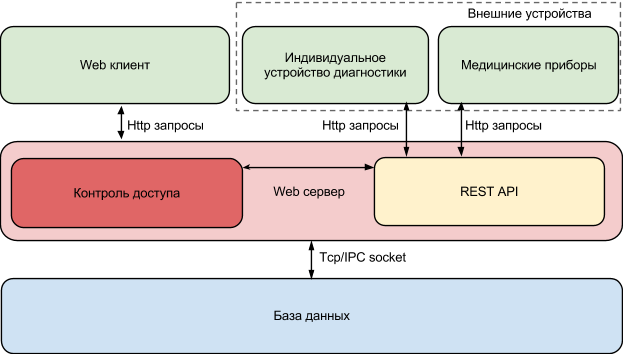
\includegraphics[width=1\linewidth]{general_architecture.eps}}
\caption{Общая архитектура системы.}
\label{ris:general_architecture}
\end{figure}

\subsection{Web клиент}
Клиент разделяет функции подсистемы ввода данных и подсистемы доступа к данным.
Основной задачей клиента является предоставление доступа к системе пользователям
с помощью веб-браузера или другого программного обеспечения способного работать
с протоколом HTTP. С точки зрения требования доступности, реализация в виде web
клиента наиболее оптимальна, так как веб-браузеры есть на всех современных
платформах и устройствах.

\subsection{Web сервер}
Основной задачей Web сервера является - организация взаимодействия между
различными клиентами и системой хранения данных. Также в рамках Web сервера
будут реализованы:
\begin{enumerate}
  \item бизнес-логика системы;
  \item контроль доступа к системе;
  \item подсистема унифицированного доступа к системе хранения данных;
  \item подсистема анализа данных;
  \item REST API для унифицированного взаимодействия с внешними источниками и
потребителями данных.
\end{enumerate}

\subsection{REST API}
Основной задачей является предоставление публичного интерфейса для ввода данных
с внешних источников.

\subsection{База данных}
Достаточно долгое время основным типом системы хранения данных была SQL база
данных. Однако в последние годы получает распространение NoSQL системы хранения.
Данные подходы к организации источника данных преследуют одну цель - обеспечить
долговременное, надежное хранение структурированных данных. Каждый подход имеет
свои преимущества и недостатки.
Для того чтобы определится какого типа будет система хранения данных необходимо
сформировать требования к системе, а затем на основании требований выбрать
наиболее подходящий тип системы.

\subsubsection{Требования к системе хранения данных}
Надежность - очень широкое понятие в терминах баз данных. Рассмотрим основные
составляющие надежной системы хранения.
\subparagraph{Обеспечение целостности данных.}
SQL системы изначально проектировались чтобы соответствовать основным принципам
ACID и как следствие предоставляют возможность хранить данные в нормализованном
виде, явно определяя связи между элементами базы даных. Однако такой подход
несет дополнительную нагрузку на базу данных, т.к. необходимо констролировать
целостность данных а базе.
NoSQL решения изначально проектировались как полная альтернатива SQL решениям.
Они позволяют хранить данные в максимально денормализованном виде. При таком
подходе вся ответственность за целостность даных возлагается целиком на
разработчиков.
\subparagraph{Масштабируемость.} 
При росте числа пользователей базы данных возникает проблема обработки большого
числа запросов к базе данных. Данную проблему можно решить за счет
горизонтальной или вертикальной масштабируемости ситемы.

При вертикальной масштабируемости предлагается обновлять конфигурацию сервера на
более современную для повышения производительности. При таком подходе очевидно
что общая производительность ситемы, если не брать в счет програмную
составляющую, ограничивается только прогресом в области производства аппаратного
обеспечения. Как правило местом преткновения становится скорость операций i/o на
жестком диске. Также стоит учитывать что цены на новинки всегда завышены и
нецелесообразно будет платить достаточно крупные суммы за повышение
производительности на несколько процентов.

При горизонтальном масштабировании предлагается распределять нагрузку на
несколько серверов баз данных. При таком подходе не нужно покупать новое
дорогостоящее оборудование, производительность не упирается в скорость i/o
операций на жестком диске, а производительность системы повышается
прямопропорционально числу серверов. Достаточно обеспечить необходимое
количество серверов чтобы балансировать нагрузку между ними.
На самом деле на этом вопрос масштабируемости не ограничивается, т.к. необходимо
учитывать еще один важный фактор - размер базы данных. Некоторые современные
базы данных поддерживают механизм партицирования. Данный механизм позволяет
разбивать таблицу на несколько частей. В результате чего возможно хранить данные
на разных носителях. Данный механиз повышает скорость доступа к данным за счет
того что выборка манипуляции с даными происходят не в контексте всей таблицы а в
контексте конкретной части таблицы. Не стоит забывать и о выборе файловой
системы под файлы базы данных и драйвера который будет управлять распределением
данных в файловой системе.
\subparagraph{Быстродействие.} 

Скорость работы подсистемы хранения данных непосредственно влияет на
продолжительность приема. Важно чтобы доступ к данным был максимально быстрым.

SQL решение накладывает некоторые ограничения. Прежде всего это индексы и
транзакции, которые могут заметно снизить скорость вставки данных, но без них
может значительно снижаться скорость выбрки данных.

NoSQL решение потенциально не имеет проблем со вставкой данных. Теоретически
вставка данных должна происходить со скоростью равной скорости записи в
оперативную память. Стоит отметить что все современные SQL базы данных
производят первичную запись данных так же в оперативную память.

\subparagraph{Выбор между SQL и NoSQL.}
Выбор между двумя подходами достаточно сложная задача. В рамках выбранной
предметной области система может быть спроектирована как NoSQL так и SQL
подходом. Однако SQL подход обеспечивает большую согласованность данных и более
простую реализацию. Так же немаловажным фактором в пользу SQL подхода является
наличие более развитых средств разработки.



\newpage
\chapter{Выбор технологий}
\subsection{В начале работы}
\subsubsection{Использование языка PHP}
Первоначально в качестве языка программирования было решено использовать язык
PHP. Это было вызвано низким порогим вхождения, его большой популярности, а
следовательно большим наличием учебных материалов и примеров.

\subsubsection{Zend Framework}
В процессе работы возникла необходимость грамотной организации исходного кода,
использование тестов. Так в проект добавилась знаменитая среди разработчиков
библиотека Zend Framework. Эта библиотека решила вопрос с организацией кода
путем использования паттерна MVC - Model View Controller.

\subsubsection{Переход на платформу ASP.NET MVC}
В процессе разработки стали заметны недостатки Zend Framework: большая
избыточность кода (много абстракций вследствие данной реализации концепции MVC),
долгое время отклика, необходимость вручную составлять запросы, связывающие
модель предметной области с базой данных.

Было решено перенести проект на стек технологий от компании Microsoft. В
качестве базовой технологии была выбрана платформа  ASP.NET, язык
программирования C\#. В качестве организации кода решено было продолжить
использовать паттерн MVC.

\subsubsection{Большие затраты времени на конфигурирование}
Вместе с использованием ASP.NET, для доступа моделей предметной области к данным
был использован паттерн Repository. Однако это не решило вопрос с ручным
созданием объектов в базе данных. Таким образом  стало ясно, что без
использования технологии ORM не обойтись. С этой целью был использована
библиотека Entity Framework.

Несмотря на то что библиотека Entity Framework сильно облегчает и ускоряет
работу программиста, регламентирование доступа к базе данных из модели с помощью
паттерна Repository заставляет писать дополнительный программный код - помимо
перечисления атрибутов сущностей в классе, для каждого поля  необходимо
прописывать атрибуты используемые в процессе работы Entity Framework.

Еще одним минусом стало ручное прописывание валидационных правил и метаданных сущностей. 
Для организации их работы приходилось вручную прописывать все атрибуты, что вызывает 
неудобство и повышает вероятность ошибки.

\subsection{Выбор платформы Ruby on Rails}
\subsubsection{Регламентированный доступ к базе данных}
Для доступа к данным в Rails используется ORM c реализацией паттерна
ActiveRecord - шаблон проектирования приложений, описанный Мартином Фаулером.
Основная суть заключается в том, что для каждой таблице в БД создается
соответствующий ей класс, каждой строке в данной таблице соответствует экземпляр
соответствующего ей класса. Каждое действие с экземпром данного класса
(создание, изменение и удаление) сопровождается соответствующими SQL- запросом.

Запросы для выборки данных создаются через Query Interface. Query Interface
представляет из себя набор классов, специфичных для каждой СУБД.

\begin{lstlisting}[language=Ruby,caption=Запрос через ActiveRecord,label={lst:ar_sample_query}] 
@appntmentEvents = 
	DoctorUser.current.appointment_events.
	where('events.status <> ?', 'free').
	order('date_start DESC')
\end{lstlisting}

В листинге \ref{lst:ar_sample_query} представлен пример запроса, который
возвращает все врачебные приемы (appointment\_events) для пользователя доктор (DoctorUser), 
который на данный момент авторизован (current)
в системе, статус которых не свободно (where('events.status <> ?', 'free')) и
сортирует их в порядке, в котором первым отображается самый поздний врачебный прием
\\ (order("date\_start DESC")).

Для изменения состава атрибутов сущности в Ruby on Rails используется инструмент
мигрирования, который будет рассмотрен ниже.

\subsubsection{Готовая система валидации вводимых данных}
Валидации используются, чтобы быть уверенными, что только верно указанные данные
сохраняются в базу данных.

В Ruby on Rails валидация реализуется с помощью предопределенных валидационных
хелперов. Эти хелперы предоставляют общие правила валидации. Каждый раз, когда
валидация проваливается, сообщение об ошибке добавляется в коллекцию errors
объекта, и это сообщение связывается с аттрибутом, который подлежал валидации.

Для того чтобы использовать валидационной хелпер, его необходимо вызвать в
классе модели и через запятую указать те атрибуты класса, которые необходимо
проверить на правильность вводимых данных.

\subsubsection{Создание связей между сущностями}
Связи между моделями нужны для облегчения выполнения обычных операций с
объектами. Среда Ruby on Rails позволяет создавать связи типа один к одному,
один ко многим и многие ко многим. В рассмотренном выше примере получения всех
врачебных приемов доктора использовалась связь appointment\_events.

Для использования связей достаточно в классе сущности указать тип связи и класс
сущности с которой создается связь. В качестве примера приведем связь между
сущностями “Событие” и “Пользователь”, которая реализуется с целью определения
пользователя-создателя события.

\begin{lstlisting}[language=Ruby,caption=Связь на
стороне события,label={lst:ar_event_links}] 
class Event < ActiveRecord::Base
  # #{Организатор события} 
  belongs_to :user
end  
\end{lstlisting}

\begin{lstlisting}[language=Ruby,caption=Связь на
стороне события,label={lst:ar_user_links}]
class User < ActiveRecord::Base  
  # #{События для которых пациент является организатором}
  has_many :events
  # #{События в которых участвовал пациент}
  has_many :attendees_events, :through => :attendees, :source => :event
end  
\end{lstlisting}

Как видно из листинга кода, сущность ``Event'' связывается связью ``oдин ко
многим'' (belobgs\_to на стороне ``одного'' и has\_many на стороне ``многие'') с сущностью
``User''.

\subsubsection{Использование соглашений по конфигурации}
Сonvention over Сonfiguration\footnote{
	\url{http://en.wikipedia.org/wiki/Convention_over_configuration}
} — это принцип построения фреймворков и
библиотек, призванный сократить количество требуемой конфигурации без потери гибкости.
Обычно переводится как «соглашения по конфигурации».
В строгой форме этот принцип можно выразить так: аспект программной системы
нуждается в конфигурации тогда и только тогда, когда этот аспект не
удовлетворяет некоторой спецификации.
В качестве примера можно привести соглашение по именованию таблиц и классов -
при формировании названия таблицы имя класса пишется со строчной буквы с
добавлением окончанием множественного числа (англ. языка) “s”.

\subsubsection{Гибкость языка Ruby}
Основное назначение Ruby — создание простых и в то же время понятных программ,
где важна не скорость работы программы, а малое время разработки, понятность и
простота синтаксиса. Язык следует принципу «наименьшей неожиданности»\footnote{
	\url{http://ru.wikipedia.org/wiki/Ruby}
}: программа должна вести себя так, как ожидает программист.

\subsubsection{Вывод}
Исходя из требований к системе, оптимальной формой интерфейса системы будет
веб-сайт. На данный момент число технологий создания веб-сайтов достаточно
велико, у каждой есть свои плюсы и минусы. Исходя из требований к технологиям
оптимальным будет выбор фрэймворка Ruby On Rails.

Основные преимущества перед другими технологиями того же уровня:
\begin{enumerate}
  \item наличие большого числа библиотек, решающих большинство типовых задач при веб-разработке;
  \item большое сообщество;
  \item быстрое развитие;
  \item простота и удобство разработки. 
\end{enumerate}

\section{Frontend}
Front-end - часть программы, которая взаимодействует с пользователем. Здесь мы
рассмотрим технологии используемые для построения графического интерфейса.

\subsubsection{Backbone.js}
Backbone.js придает структуру веб-приложениям с помощью моделей с биндингами по
ключу и пользовательскими событиями, коллекций с богатым набором методов с
перечислимыми сущностями, представлений с декларативной обработкой событий; и
соединяет это все с существующим REST-овым JSON API\footnote{
	\url{http://backbonejs.ru/}
}.

При использовании backbone.js данные предметной области представляются как
Модели (Models), которые могут быть созданы, провалидированы, удалены, и
сохранены на сервере. Всякий раз, когда в интерфейсе изменяется атрибуты модели,
модель вызывает событие "change"; все Представления (Views), которые отображают
состояние модели, могут быть уведомлены об изменении атрибутов модели, с тем
чтобы они могли отреагировать соответствующим образом — например, перерисовать
себя с учетом новых данных.

Основной полезный эффект возникающий от добавления backbone.js в проект
заключается в том, что разработчику не надо писать код, ищущий элемент с
определенным id в DOM и обновляющий HTML вручную. При изменении модели
представление просто обновит себя самостоятельно.

\subsubsection{Coffeescript}
Встроенная поддержка CoffeeScript была добавлена в Rails с версии 3.1. Программы
написанные на данном языке перед выполнением компилируются в javascript. Язык
CoffeeScript позволяет писать программы в функциональном стиле, в нем более
полно реализовано использование классов.

CoffeeScript используется чтобы улучшить читаемость кода и уменьшить его размер.
В среднем для выполнения одинаковых действий на CoffeeScript требуется в 2 раза
меньше строк, чем JavaScript\footnote{
	\url{http://coffeescript.org/}
}.

\subsubsection{RequireJs}
При разработке приложений с модульной структурой на JavaScript возникает две
проблемы:
\begin{enumerate}
  \item описание и удовлетворение зависимостей различных частей приложения, необходимость организации подключения зависимостей на серверной стороне;
  \item экспорт переменных в глобальную область видимости и их коллизия. 
\end{enumerate}

Озвученные проблемы можно решить используя фреймворк RequireJs. В этом случае на
странице достаточно использовать только один тег <script>. Все остальные js
файлы и библиотеки подключаются при вызове главной функции define. Пути к
подключаемым файлам передаются данной функции в качестве аргументов, а
возвращаемым значением будет являться весь javascript-контекст веб-страницы.

Подключаемым файлам необходимо назначить уникальное имя, по которому к нему
будет происходить обращение в результирующей функции (define).

\subsubsection{Twitter Bootstrap}
Для быстрой разработки интерфейса хорошо зарекомендовала себя библиотека (UI
Framework) Twitter Bootstrap. Framework содержит набор стилей CSS и javascript
функций, а также регламентирует варианты html разметки страницы: таблицы,
кнопки, стикеры, уведомления и многое другое. Для использования библиотеки
достаточно подключить несколько css стилей и javascript файлов. Далее при
создании веб-страниц для использования данной библиотекой для используемых тегов
достаточно указать необходимые значения атрибута class. Таблицу со значениями
атрибутов можно найти на официальном сайте\footnote{
	\url{http://twitter.github.io/bootstrap/}
}.

\subsubsection{Ресурсы приложения}
В Ruby on Rails все стили, скрипты js, картинки хранятся в папке app/assets. В
Ruby on Rails скрипты пишутся на языке coffee-script, а стили на SASS. В рабочем
режиме (production) исходные коды на этих языках компилируются в обычные CSS и
javacript файлы и затем на все входящие запросы отдаются как статичные файлы,
непосредственно веб-сервером. Благодаря такому подходу снижается нагрузку на
серверную машину, а следовательно уменьшается время отклика. В режиме
разработчика (development) перекомпиляция происходит при каждом запросе, для
оперативного просмотра изменений в исходном коде в процессе разработки.

\subsubsection{Средство построения графиков}
Основной целью разрабатываемой информационной системы является мониторинг
состояния здоровья пациентов. Основным средством визуального отображения
результатов мониторинга являются информационные графики и диаграммы. Для вывода
графиков используется javascript библиотека Highcharts\footnote{
	\url{http://www.highcharts.com/}
}.

\subsection{Backend}
В данном разделе рассмотрены технологии, с которыми пользователь непосредственно
не взаимодействует. Поскольку разрабатываемая нами информационная система
является клиент-серверным веб-приложением, здесь будет рассмотрена так
называемая серверная компонента.

\subsubsection{Ruby}
Создатель Ruby — Юкихиро Мацумото (Matz) — интересовался языками
программирования, ещё будучи студентом, но идея о разработке нового языка
появилась позже. Ruby начал разрабатываться 23 февраля 1993 года и вышел в свет
в 1995 году.

Название навеяно языком Perl, многие особенности синтаксиса и семантики из
которого заимствованы в Ruby: англ. pearl — «жемчужина», ruby — «рубин».

Целью разработки было создание «настоящего объектно-ориентированного», лёгкого в
разработке, интерпретируемого языка программирования.

Язык следует принципу «наименьшей неожиданности»: программа должна вести себя
так, как ожидает программист.

\subsubsection{Ruby on Rails}
Фреймворк Ruby on Rails был создан Давидом Хейнемейером Ханссоном на основе его
работы в компании 37signals над средством управления проектами Basecamp и
выпущен в июле 2004 года.

Ruby on Rails определяет следующие принципы разработки приложений:

\begin{enumerate}
  \item предоставляет механизмы повторного использования, 
позволяющие минимизировать дублирование кода в приложениях (принцип Don’t repeat yourself);
  \item по умолчанию используются соглашения по конфигурации, типичные для
большинства приложений (принцип Convention over configuration).
\end{enumerate}

\subsubsection{Концепция MVC}
Основными компонентами приложений Ruby on Rails являются модель (model),
представление (view) и контроллер (controller). Ruby on Rails использует
REST-стиль построения веб-приложений.

\subparagraph{Модель} 
Модель предоставляет остальным компонентам приложения объектно-ориентированное
отображение данных (таких как каталог продуктов или список заказов). Объекты
модели могут осуществлять загрузку и сохранение данных в реляционной базе
данных, а также реализуют бизнес-логику.

Как уже говорилось выше, для хранения объектов модели в реляционной СУБД по
умолчанию в Rails 3 использована библиотека ActiveRecord. Конкурирующий аналог —
DataMapper. Существуют плагины для работы с нереляционными базами данных,
например Mongoid для работы с MongoDB.

В качестве примера модели рассмотрим сущность Документ (листинг
\ref{lst:document_model_example} .  Как видно, в начале кода описывающего модель вводятся связи с другими сущностями (в данном
случае это пользователь создавший документ и событие к которому документ
привязан). После этого описывает валидация, затем вводятся так называемы
коллбэки - функции которое будут вызваны в случае инвольвинга определенных
событий. В данном случае перед созданием экземплера документа, в качестве
создателя будет записан текущий пользователь.

\begin{lstlisting}[language=Ruby,caption=Модель документов
,label={lst:document_model_example}] 
class Document < ActiveRecord::Base
  # #{Создатель документа}
  belongs_to :user
  # #{Событие к которому привязан документ}
  belongs_to :event

  attr_accessible :event_id

  validates :user_id, :presence => true

  # #{Назначем создателем события текущего авторизованного пользователя}
  before_create do
    if User.current.present?
      self.user_id = User.current.id
    end
  end
end
\end{lstlisting}

\subparagraph{Представление}
Представление создает пользовательский интерфейс с использованием полученных от
контроллера данных. Представление также передает запросы пользователя на
манипуляцию данными в контроллер (как правило, представление не изменяет
непосредственно модель).

В Ruby on Rails представление описывается при помощи шаблонов ERB. Они
представляют собой файлы HTML с дополнительными включениями фрагментов кода Ruby
(Embedded Ruby или ERb). Вывод, сгенерированный встроенным кодом Ruby,
включается в текст шаблона, после чего получившаяся страница HTML возвращается
пользователю. Кроме ERB возможно использовать ещё около 20 шаблонизаторов, в том
числе Haml.

Пример представления приведен в листинге \ref{lst:view_example}. В данном
примере показано представление, отрисовывающее главную страницу. Проверяется условие - если
пользователь зарегестрирован - то отрисвывается ссылка на личный кабинет
пользователя, иначе отрисовывается общая информация.

\begin{lstlisting}[language=Ruby,caption=Страница приветствия
,label={lst:view_example}] 
<% if user_signed_in? %>
    <h1>#{Начать работу}</h1>
    <p>#{В личном кабинете вы можете:}</p>

    <%= render :partial => '/cabinets_list' %>
<% else %>
    <div class="hero-unit">
      <h1>#{Начать работу}</h1>
      <p>....</p>
      <p>
        <a class="btn btn-primary btn-large" href="<%= new_user_session_path() %>">
          #{Войти}
        </a>
      </p>
    </div>

    <div class="hero-unit">
      <h1>#{Впервые на сайте?}</h1>
      <p>....</p>
      <p>
        <a class="btn btn-primary btn-large" href="<%= new_bid_path() %>">
          #{Регистрация}
        </a>
      </p>
    </div>
<% end %>
\end{lstlisting}

\subparagraph{Контроллер.}
Контроллер в Rails — это набор логики, запускаемой после получения HTTP-запроса
сервером. Контроллер отвечает за вызов методов модели и запускает формирование
представления.

Соответствие url адреса и контроллера задается в файле config/routes.rb.

Контроллером в Ruby on Rails является класс, наследованный от \\
ActionController::Base. Открытые методы контроллера являются так называемыми
действиями (actions). Action часто соответствует отдельному представлению.
Например, по запросу пользователя admin/list будет вызван метод list класса
AdminController и затем использовано представление \\ list.html.erb.

Пример кода контроллера приведен в листинге \ref{lst:controller_example}. На
данном рисунке хорошо демонстрируется суть контроллера - соединить поступивший HTTP-запрос (params) с
моделью предметной области.

\begin{lstlisting}[language=Ruby,caption=Контроллер для приема диагностики
,label={lst:controller_example}] 
class Cabinet::Doctor::DiagnosticController < Cabinet::DoctorController
  def show
    @patient = PatientUser.find(params[:id])
  end

  def chart
    from = Time.at(params[:from].to_i)
    to = Time.at(params[:to].to_i)

    respond_to do |f|
      f.json { 
      	render json: ChartFactory.build(params[:patient_id], params[:parameter_id], from, to) 
      } 
    end
  end

  def raw
    from = Time.at(params[:from].to_i)
    to = Time.at(params[:to].to_i)
    @data = DiagnosticFactory.raw(params[:patient_id], params[:parameter_id], from, to)
  end
end
\end{lstlisting}

\subsection{Дополнительные возможости платформы Ruby on Rails}
\subsubsection{Встроенный генератор Rails Generator}
Использование генератора Rails сопровождает разработчика с момента инициализации
нового проекта. Генератор - это скриптовая программа на языке Ruby, которая на
основе полученных входных данных генерирует на основе шаблонов стандартные файлы
исходного кода проекта. Это избавляет разработчика от рутинной работы по
созданию файлов и папок, которые стандартны для всех проектов Rails.
Классический пример использования представлен в листинге
\ref{lst:rails_new_application}  - инициализация нового проекта .

\begin{lstlisting}[language=Bash,caption=Создание
нового приложения,label={lst:rails_new_application}] 
user@host$ rails generate some_application_name
\end{lstlisting}

\subsubsection{Формы ввода данных}
Формы в веб-приложениях – это основной интерфейс для пользовательского ввода.
Однако, обработка форм может достаточно трудоемкой из-за необходимости описывать
элементы форм, правила валидации данных на стороне клиента и сервера. Rails
устраняет эти сложности, предоставляя хелперы для разметки форм. Помимо
стандартных хелперов, существует библиотека simple\_form. Данная библиотека
сокращает время при написании кода веб-формы, а именно - разработчику не нужно
указывать URL-адрес обработчика запроса (при нажатии кнопки submit); не нужно
вручную прописывать HTML-разметку для элемента, отвечающего за отображение и
хранение значения того или иного атрибута - алгоритм simple\_form сам подберет
необходимую разметку на основании типа данных. Кроме того simple\_form сама
преобразует существующую валидацию (реализованную средствами Rails) в валидацию
на стороне клиента (работающую на javascript). Это дает очевидную выгоду -
поскольку ошибки отсекаются на стороне клиента, снижается нагрузка на сетевое
соединение и на обрабатывающий сервер.

\subsubsection{Рассылка  электронной почты}
Action Mailer позволяет отправлять электронные письма из приложения, используя
модель и представления рассыльщика. Таким образом, в Rails электронная почта
используется посредством создание рассыльщиков, наследуемых от
ActionMailer::Base, и находящихся в app/mailers. Эти рассыльщики имеют связанные
представления, которые находятся среди представлений контроллеров в app/views.

Для рассылки почты не требуется приобретение и развертывание собственного
почтового сервера. Достаточно подключить существующий аккаунт в популярных
почтовых серверах (yandex, gmail) в конфигурационных файлах
(config/environments/production.rb) приложения. Веб-сервер будет отсылать
электронные письма подключившись к аккаунту через протокол SMTP.

В режиме разработчика (development) можно настроить имитацию отправки писем для
проверки правильности работы мейлера и тестирования системы в целом. В этом
случае веб-сервер будет сохранять отправляемые письма в виде файлов, в папку
tmp.

\subsubsection{Система контроля версий базы данных}
Поскольку очень часто (как и в нашем случае) разработчики работают в команде,
возникает проблема контроля версий. Причем данный контроль должен выполняться не
только в отношении исходного кода и задач (см. git, github), но и за состоянием
структуры базы данных.

Данная проблема успешно решается с помощью концепции мигрирования БД. Она
заключается в том, что все изменения базы данных делятся на фрагменты -
миграции.

В первых версиях фреймворка Rails разработчик должен был сам назначить имя
миграции. Это часто приводило к коллизиям и приходилось вручную менять и
миграцию и структуру БД.

В более поздних версиях к имени миграции стал добавляться хэш отражающий дату
создания миграции.

C помощью выбранной системы контроля версий разработчики синхронизируют файлы
миграций между собой и рабочим сервером (рис. \ref{ris:development_migrations}).

Active Record отслеживает, какие миграции уже были выполнены, поэтому все, что
нужно сделать, это обновить свой исходный код и запустить rake db:migrate.
Active Record сам определит, какие миграции нужно запустить, проверив таблицу
базы данных schema\_migrations, автоматически создаваемую при изначальном вызове
rake db:migrate. schema\_migrations содержит единственный столбец с именем
versions, содержащий временные метки, с которых начинаются созданные миграции
Active Record (рис. \ref{ris:migration_algorithm}). Каждая временная метка,
содержащаяся в schema\_migrations, показывает, что миграция, связанная с временной меткой, была
вызвана ранее, и не должна быть вызвана при будующих вызовах rake db:migrate. Он
также обновит файл db/schema.rb в соответствии с новой структурой базы данных.

\begin{figure}[h]
\center{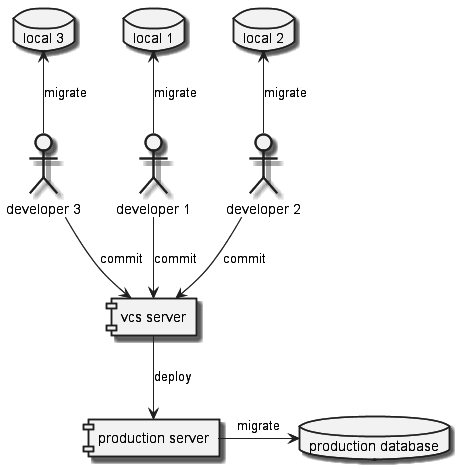
\includegraphics[width=0.5\linewidth]{development_migrations.eps}}
\caption{Централизованный контроль версий базы данных.}
\label{ris:development_migrations}
\end{figure}

\begin{figure}[h]
\center{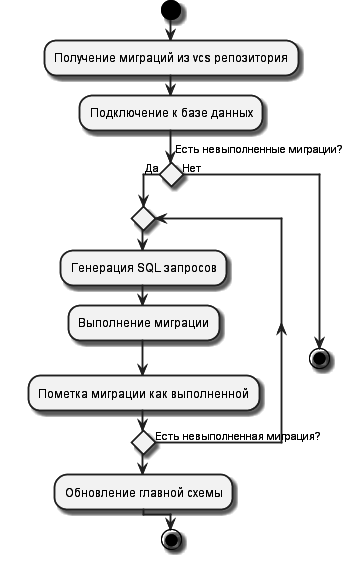
\includegraphics[width=0.5\linewidth]{migration_algorithm.eps}}
\caption{Схема выполнения миграции.}
\label{ris:migration_algorithm}
\end{figure}

\subsection{Использование сторонних библиотек на языке Ruby}
В процессе разработки проекта для решения многих типовых задач также были
использованы библиотеки из хостинга RubyGems. Как правило для каждой задачи
используется соответствующая библиотека (или группа библиотек). Перечень всех
библиотек находится в файле Gemfile. Для установки библиотек на компьютер
разработчика, а также на рабочую машину системы производится с помощью
специальной утилиты Bundler, которая читает перечень гемов из Gemfile, скачивает
необходимые библиотеки с хостинга и выполняет постинсталляционные скрипты. После
установки всех необходимых библиотек Bundler фиксирует версию каждой библиотеки
в файле Gemfile.lock. Фиксирование версий библиотек позволяет снижать риск
несовместимости между библиотеками при развертывании приложения на рабочем
сервере.

\subsubsection{Аутентификация и авторизация}
Данная задача была самой первой и ее причины очевидны - обработка личной
медицинской информации предполагает тщательной сохранение медицинской тайны.
Разграничение прав доступа к данным и функционалу также крайне необходимы -
недопустимо чтобы доктор мог изменять значения, введенные пациентом. В то же
время некоторые сведения о пациентах и о других пользователях могут быть
изменены (например, фамилия).
Проанализировав эти и другие требования (такие как простота и стоимость
реализации) мы пришли к выводу что для организации функции аутентификации и
аутентификации необходимо использовать стороннюю библиотеку devise, а для
функции авторизации библиотеку CanCan.

\subsubsection{Доступ к базе данных}
Для взаимодействия с хранилищем данных проект на Ruby on Rails использует
специальные библиотеки. Для каждой СУБД существует своя библиотека подключений.
В нашем проекте использует Postgresql 9.1 (подробнее см. ниже). Для подключения
к данной СУБД существует библиотека pg.
    
Среда Rails для манипулирования данными вызывает функции из этой библиотеки,
далее внутри в библиотеки происходит их преобразование в sql и далее запрос
отправляется к СУБД. Данные для подключения библиотека берет из файла
конфигурации.

\subsubsection{Служебная утилита rake}
Rake\footnote{
	\url{http://ru.wikipedia.org/wiki/Rake}
} — инструмент для автоматизации сборки программного кода. Он подобен
SCons, Make и Apache Ant, но имеет несколько отличий. Этот инструмент написан на языке
программирования Ruby. Автором Rake является Jim Weirich.
Rake использует блоки анонимных функций Ruby для определения различных задач,
используя синтаксис Ruby. В нем есть библиотека основных заданий, таких как
функции для задач манипулирования файлами и библиотека для удаления
скомпилированных файлов (задача «очистки»). Как и Make, Rake может также
синтезировать задачи, основываясь на шаблонах (например, автоматическая сборка
задачи компилирования файла на основе шаблонов имен файлов).
При работе с Ruby on Rails утилита rake занимает особое место. С помощью данной
утилиты выполняется много служебных действий как в режиме разработчика, так и на
рабочей машине. С помощью данной утилиты происходит выполнение миграции и запуск
websocket сервера.

\begin{lstlisting}[language=Bash,caption=Выполнение миграций
,label={lst:rails_new_application}] 
user@host$ rake db:migrate
\end{lstlisting}

\begin{lstlisting}[language=Bash,caption=Компиляция ресурсов
,label={lst:rails_new_application}] 
user@host$ rake assets:precompile
\end{lstlisting}
 
 Данная команда запустит процедуру компиляции материалов веб-страниц на рабочей
 машине (см. раздел fronted).
 
 \subsubsection{Тестирование отправки писем}
 Для этого используется библиотека mailcatcher. По сути это простейший
 SMTP-сервер который перехватывает письма и позволяет просматривать их с помощью
 веб-интерфейса.
 
 \subsection{Postgresql}
Основными критериями при выборе СУБД были: открытость, функциональность и
наличие опыта работы с данной базой данных, а так же простота интеграции с
выбранным стеком технологий. Выбор был сделан в пользу Postgresql.

Для работы с Postgresql для Ruby On Rails существует библиотека pg, реализующая
Active Record Query Interface специфичный для Postgresql.

Данная база данных достаточно надежна и проста в обращении.

Основные преимущества:
\begin{enumerate}
  \item GNU General Public License;
  \item встроенный механизм полнотекстового поиска;
  \item простая реализация резервного копирования базы в реальном времени;
  \item наличие готовых средств для баллансировки нагрузки;
  \item с версии 9.0 поддерживается потоковая репликация (Hot Standby);
  \item транзакционный DDL.
\end{enumerate}

\subsection{Websocket}
Одной из целью создания системы является - постоянный обмен актуальной
информацией о состоянии пациента.
	
Websocket сервер позволить организовать это взаимодействие в реальном времени с
минимальными задержками, за счет возможности инициировать передачу информации с
backend во frontend на стороне backend.
	
Для работы с Websocket сервером используется одноименный протокол WebSocket\footnote{
	\url{http://ru.wikipedia.org/wiki/WebSocket}
}.

Основной задачей Websocket сервера является оповещение подписчиков о наступлении
определенного события и отправке подписчикам метаданных связанных с событием.
Событием в рамках приложения может быть:
\begin{enumerate}
  \item любая CRUD операция над моделью;
  \item выполнение какого-либо бизнес-процесса.
\end{enumerate}

Реализация Websocket сервера базируется на библиотеке Eventmachine\footnote{
	\url{http://rubyeventmachine.com/}
}. В текущей реализации Websocket сервер позволяет выполнять следующие операции:
\begin{enumerate}
  \item присоединение/отсоединение клиента от определенного канала;
  \item передача сообщений как в рамках определенного канала, так и
широковещательных сообщений.
\end{enumerate}

На стороне клиента используется стандартный объект WebSocket обернутый в класс
на CoffeeScript для более удобной работы.

\newpage
\chapter{Организация процеса разработки}
\subsection{Определение условий разработки}
В связи с тем, что разработка проекта ведется в команде, необходимо решить
проблему совместного доступа к файлам проекта. Помимо этого, файлы проекта во
время работы постоянно претерпевают различные изменения. При этом часто бывает
важно иметь не только последние версии, но и несколько предыдущих. В простейшем
случае можно просто хранить несколько вариантов документа, нумеруя их
соответствующим образом. Такой способ неэффективен (приходится хранить несколько
практически идентичных копий), требует повышенного внимания и дисциплины и часто
ведёт к ошибкам, поэтому были разработаны средства для автоматизации этой
работы. В качестве решения данной проблемы неэффективности было решено
использовать системы управления версиями (VCS -  Version Control System).

\subsection{Система управления версиями Git}
Данная система  спроектирована как набор программ, специально разработанных с
учётом их использования в скриптах. Это позволяет удобно создавать
специализированные системы контроля версий на базе Git или пользовательские
интерфейсы.
Достоинствами данной системы являются:
\begin{enumerate}
  \item высокая производительность;
  \item децентрализованность;
  \item развитые средства интеграции с IDE;
  \item продуманная система команд.
\end{enumerate}

\subsection{Веб-сервис GitHub}\footnote{
	\url{https://github.com/}
} 
Это веб-сервис для хостинга проектов и их совместной разработки. GitHub
позиционируется как веб-сервис хостинга проектов с использованием системы
контроля версий git, а также как социальная сеть для разработчиков. Пользователи
могут создавать неограниченное число публичных репозиториев, для каждого из
которых предоставляется wiki, система issue tracking-а, есть возможность
проводить code review и многое другое. GitHub на данный момент является самым
популярным сервисом такого рода, обогнав Sourceforge и Google Code.

\subsection{Организация документации по проекту}
В процессе разработки проекта вместе с кодом создаются файлы документации. К ним
можно отнести документы разработки (записи требований заказчика, планы, отчеты о
ходе разработки), схемы, диаграммы и графические модели предметной области и пр.
В связи с этим возникает необходимость организации совместного доступа и
хранения данных файлов.

\subsubsection{Веб-приложение  Google Docs}
Данное приложение представляет из себя бесплатный онлайн-офис, включающий в себя
текстовый, табличный процессор и сервис для создания презентаций, а также
интернет-сервис облачного хранения файлов с функциями файлообмена,
разрабатываемый компанией «Google». Данный сервис также позволяет одновременное
совместное редактирование файлов.

\subsubsection{Веб-приложение diagram.ly}
Приложение позволяет создавать диаграммы различного типа. Поддерживает интеграцию с Google Docs.

\subsubsection{XMind}
XMind — это открытое программное обеспечение для проведения мозговых штурмов и
составления интеллект-карт, разрабатываемое компанией XMind Ltd.

Эта программа помогает пользователю фиксировать свои идеи, организовывать их в
различные диаграммы, использовать эти диаграммы совместно с другими
пользователями. XMind поддерживает интеллект-карты, диаграммы Исикавы (также
известные как fishbone-диаграммы или причинно-следственные диаграммы),
древовидные диаграммы, логические диаграммы, таблицы.

\subsubsection{Plant UML}\footnote{
	\url{http://plantuml.sourceforge.net/}
}
Plant UML - это открытое програмное обеспечение для постороения UML-диаграмм.
Важная особенность работы с Plant UML состоит в том, что любые диаграммы можно
описать на специальном языке в текстовой форме, после чего получить диаграмму в
виде png или svg файла.

\newpage
\chapter{Разработка проекта}
\subsection{План разрабоки}\footnote{
	\url{https://github.com/crashr42/shm/issues/milestones}
}
Процесс разработки разбит на несколько фаз. Фаза состоит из предварительного
набора задач по завершению которых  фаза будет считаться завершенной.

\subsubsection{Skeleton}
Цель - настройка среды для разработки, построение простейшего "скелета" системы:
\begin{enumerate}
  \item установка и настройка ruby, rvm, rails;
  \item установка и настройка postgres;
  \item инициализация проекта;
  \item настройка авторизации;
  \item установка админки.
\end{enumerate}

\subsubsection{General}
Цель - разрабока основы предметной области, доработка каркаса приложения:
\begin{enumerate}
  \item отражение основных объектов предметной области в виде классов моделей;
  \item покрытие тестам;
  \item организация стурктуры для js клиета.
\end{enumerate}

\subsubsection{Patient}
Цель - реализовать кабинет пациента:
\begin{enumerate}
  \item профиль;
  \item запись на прием;
  \item рассписание приемов у врача;
  \item рассписание приема лекарств;
  \item рассписание ввода показателей здоровья.   
\end{enumerate}

\subsubsection{Manager}
Цель - реализовать кабент менеджера:
\begin{enumerate}
  \item просмотр заявок;
  \item подтверждение заявок;
  \item отклонение заявок.   
\end{enumerate}

\subsubsection{Patient/Doctor}
Цель - организация взаимодействия между доктором и пациентом:
\begin{enumerate}
  \item общение пациента с доктором;
\end{enumerate}

\subsubsection{Doctor}
Цель - разработка кабинета доктора:
\begin{enumerate}
  \item просмотр своих пользователей;
  \item электронный прием;
  \item электронная запись на прием;
  \item назначение лекарств;
  \item назначение диагнозов;
  \item визуализация данных за период времени;
  \item отчеты.
\end{enumerate}


\subsection{Git Workflow}
Git Workflow - это методология организации работы с репозиторием исходного кода.
Особенностью методологии является необходимость создавать отдельную ветку под
каждую задачу (issue-82, issue-85). Так же в репозитории присутствует хотя бы
одна центральная ветка (master) в которую сливаются изменения из ругих веток. В
крупных проектах могут присутствовать дополнительные центральные ветки,
предназначенные для объединения изменений перед тестированием продукта или
объединения изменений в процессе разработки. Введение дополнительных веток
позволяет работать на рабочей версией кода не обращая внимания на текущее
состояние разработки.

\begin{figure}[h]
\center{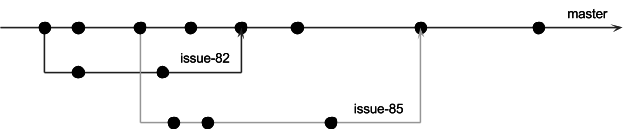
\includegraphics[width=1\linewidth]{one_central_branch.eps}}
\caption{Схема с одной центральной веткой.}
\label{ris:one_central_branch}
\end{figure}

В проекте использовались дополнительные центральные ветки для организации работы
над отдельной фазой. Со временем стало понятно что вести разработку в таком виде
сложно из-за того что необходимо было синхронизировать изменения в нескольких
центральных ветках. Так как проект еще не имел релизной версии, было принято
решение использовать одну центральную ветку (master) для всех задач (рис.
\ref{ris:one_central_branch}).

\subsection{Rails Style Guide}
При разработке Ruby On Rails приложений необходимо соблюдать определенный стиль при написании кода. Соблюдение единого стиля позволяет исключить ряд проблем связанных с коллективной разработкой.

Во-первых регламентируется форматирование кода единое для всех разработчиков.
Данный регламент позволяется исключить незначительные изменения в коммитах,
делая их более согласованными.

Во-вторых регламентируются правила работы со встроенными компонентами фрэймворка
Ruby On Rails, такими как:
\begin{enumerate}
  \item конфигурация приложения;
  \item роутинг;
  \item контроллеры;
  \item модели;
  \item ORM;
  \item миграции;
  \item локализация;
  \item установка дополнительных библиотек.   
\end{enumerate}

Соблюдение данных регламентов позволяет писать качественный код понятный другим
разработчикам.

\section{Физическое проектирование базы данных}
В процессе разработки возник вопрос как организовать физическое изменение
структуры базы данных. Классический подход создания структуры базы данных для
конкретной СУБД - код на языке SQL. Такой подход удобен если структура базы
создается единожды и не меняется в процессе разработки. На практике структура
базы данных меняется очень часто. Ситуация усугубляется если структуру базы
данных могут менять несколько разработчиков одновременно. Система контроля
версий может решить данную проблему, но лишь частично.

\subsubsection{Миграции}
Ruby On Rails предлагает встроенный механизм миграций. Миграции - это
методолигия позволяющая решить проблему изменения структуры базы данных при
разработке. Миграция представляет собой код, способный изменить структуру базы
данных.
Основные идеи:
\begin{enumerate}
  \item изменения в структуре базы данных должны быть атомарными;
  \item каждое атомарное изменение оформляется в виде миграции;
  \item должна быть возможность возвращать структуру базы данных к выбранному
состоянию.
\end{enumerate}

Каждая миграция снабжается временной меткой, характеризующей время создания
миграции. По этим временным веткам происходит упорядочивание порядка выполенения
миграций. Фиксация выполненных миграций производится на уровне базы данных в
специальной таблице “schema\_migrations”. В таблицу заносятся временные метки
выполненных миграций.

\begin{lstlisting}[language=Ruby,caption=Пример миграций
,label={lst:migration_example}] 
class CreateBids < ActiveRecord::Migration
  def change
    create_table :bids do |t|
      t.string      :first_name,    :null => false
      t.string      :last_name,     :null => false
      t.string      :third_name,    :null => true
      t.string      :address,       :null => false
      t.string      :policy,        :null => false
      t.string      :passport_scan, :null => false
      t.string      :status,        :null => false, :default => 'created'
      t.timestamps
    end
  end
end
\end{lstlisting}

В листинге \ref{lst:migration_example} представлен пример миграции, создающей в
базе данных таблицу для хранения заявок на регистрацию.

\subsection{Тестирование}
Для контроля верности выполнения бизнес-процессов в проекте используется unit
тестирование с помощью библиотеки RSpec. Такой подход позволяет иключать
логические ошибки без полноценного запуска системы, как следствие повышается
скорость разработки.

Для удобства и автоматизации тестирования применяется концепция автоматического
тестирования. При каждом изменении в коде, если для данного изменения есть тест,
тест запускается и выводится уведомление о результате выполнения теста. Для
организации данного подхода используется библиотека Autotest.

Еще один ньюанс который нужно учитывать при тестировани заключается в том что
Ruby On Rails окружение запускается достаточно долго из за этого в несколько раз
увеличивается время выполнения тестов. Для решения данной проблемы используется
библиотека Spork. Spork запускает окружение Ruby On Rails и исключает
необходимость перезапускать окружение каждый раз. Так же Spork автоматически
перезагружает классы при изменении их исходного кода.
\newpage
\ESKDthisStyle{formII}
\section{Описание системы}
\subsection{Выделенные сущности}
При создании концептуальной модели предметной области, мы выявили состав
логических сущностей (см. раздел \ref{sec:analize_subject_area}).

В процессе разработки и  проводимых нами исследований, этот набор сущностей плавно
перешел в набор классов, которые представляют эти сущности в программной среде.
Приложение \ref{app:class_diagramm}

\subsection{Кабинеты}
Весь функционал системы распределен по личным кабинетам - самостоятельным
(реализация каждого модуля независима друг от друга) javascript-приложениям.
Данное распределение позволяет сделать систему понятной, безопасной, уменьшается
избыточность исходного кода.

После авторизации на главной странице, пользователь переходит по ссылке в свой
личный кабинет. Основная навигация происходит с помощью верхнего меню.

Доктор в своем кабинете может открыть список пациентов (приложение
\ref{app:doctor_cabinet_patients}) и кликнув на конкретного пациента в списке
получает возможность работать с его учетной записью:
просмотреть и указать диагноз, просмотреть список лекарств (приложение
\ref{app:doctor_cabinet_medicament}) которые принимает пациент, назначить
пациенту врачебный прием, а также записать пациента на обследование к другому
доктору.

Одним из видов коммуникации между пациентом и доктором в системе является
врачебный прием (приложение \ref{app:doctor_cabinet_appointments}). Помимо
возможности записи на прием, в кабинете доктора есть страничка приема. В момент
когда пациент заходит в приемный кабинет, доктор (или его ассистент) должен
нажать кнопку “Начать прием”, при этом будет отмечено фактическое начало приема.
После этого в системе становится доступным отмена или назначение приема лекарств
пациенту. По окончании приема необходимо нажать кнопку “Завершить прием”. При
необходимости доктор составляет документ по результатам приема.

В кабинете пациента доступно расписание событий, которые назначены пациенту. Как
правило это приемы у врача, лечебные процедуры, уведомления о приеме лекарств.
Также у пациента есть возможность выбрать лечащего врача.

Основной функцией пользователя-пациента является дистанционная подача  значений
своих медицинских параметров в медицинское учреждение. Это производится путем
ввода информации в специальные веб-формы. Доктор в своем личном кабинете имеет
возможность просматривать значений параметров указанные его пациентами, а также
может ознакомиться с результатами аналитики, которые представлены в виде таблиц,
графиков и диаграмм.

В кабинете менеджера находится панель управления всеми пользователями системы.
Также одной из функций менеджера является рассмотрение заявок на регистрацию
нового пользователя в системе.

Если пациент хочет принять участие в проекте, то он должен заполнить заявку на
регистрацию. В ней он указывает свои учетные данные медицинского учреждения
(номер страхового полиса, больничной карты), а также прикладывает
отсканированное изображение паспорта.

Менеджер системы просматривает поступившие заявки, проверяет верность указанных
в них данных и либо создает нового пользователя, либо отклоняет заявку.
\subsection{События}
В системе реализована событийная модель, характеризующая реальные процессы:
прием, обследование. Базовам классом для всех событий является класс Event.
Событие может находиться в 4 состояниях:
\begin{enumerate}
  \item free - событие доступо для работы (например на прием у врача со статусом
  free можно записаться); 
  \item busy - событие занято (например на прием к врачу со статусом busy
  записаться не получится); 
  \item process - событие обрабатывается (врач ведет прием пациента);
  \item close - событие завершено (прием окончен).   
\end{enumerate}

Статус события может меняться только в определенном порядке:
\begin{enumerate}
  \item free -> busy (запись на прием);
  \item busy -> free (освободить запись);
  \item busy -> process (начать прием);
  \item process -> close (завершить прием).
\end{enumerate}

Такой подход обусловлен тем что с каждым переходом может быть связано
определенное действие. Если не фиксировать возможные переходы, то для перехода,
например, со статуса free -> close нужно будет создавать дополнительный
обработчик.

Для контроля смены статуса событий и создания обработчиков этих переходов был
создан модуль Workflow. Реализация в виде модуля обусловлена тем что позволяет
внедрять данный модуль в любой класс. Пример использования модуля для обработки
переходов для событий приведен в листинге \ref{lst:using_workflow_module}.

\begin{lstlisting}[language=Ruby,caption=Использование модуля Workflow
,label={lst:using_workflow_module}] 
class Event < ActiveRecord::Base
  include Workflow

  # #{Возможные переходы для статуса события}
  workflow :status do
    flow :default, :busy => :process
    flow :default, :process => :close

    flow :reset_duration, :free => :busy do
      if self.event.present?
        self.event.duration -= self.date_end - self.date_start
      end
      self.duration = 0
    end

    flow :reset_duration, :busy => :free do
      if self.event.present?
        self.event.duration += self.date_end - self.date_start
      end
      self.duration = self.date_end - self.date_start
    end
  end
end
\end{lstlisting}
\section{Диагностика}
\subsubsection{Прием данных}
Прием диагностических данных в системе осуществляется через отсылку запроса на
REST API. Запрос представляется из себя стандартный POST запрос по адресу
\url{http://localhost:3000/diagnostic/parameter} (листинг
\ref{lst:sending_diagnostic}) с указанием дополнительных параметров:
\begin{enumerate}
  \item user\_id - идентификатор пользователя в системе;
  \item parameter\_id - идентификатор мараметра;
  \item value - значение параметра.   
\end{enumerate}

\begin{lstlisting}[language=Bash,caption=Отправка диагностических данных
,label={lst:sending_diagnostic}] 
user@localhost$ curl -d "user_id=1&parameter_id=2&value=44" \
http://localhost/diagnostic/parameter
\end{lstlisting}

\subsubsection{Доступ к диагностическим данным}
Доступ к диагностическим данным предоставляется доктору. Доктор может
просматривать данные в виде графиков или таблиц. Графики формируются с помощью
класса ChartFactory в зависимости от класса параметра. ChartFactory имеет метод
build который принимет в качестве параметров:
\begin{enumerate}
  \item patient\_id - идентификатор пациента;
  \item parameter\_id - идентификатор параметра;
  \item from - начальная дата для выборки данных;
  \item to - конечная дата для выборки данных.
\end{enumerate}

Метод возвращает ассоциативный массив со структурой понятной \\ Highcharts.
После чего массив сериализуется в JSON и отдается клиенту.

\subsubsection{События}
После поступления диагностических данных в систему, системы инициирует
специальное событие. Событие указывает Websocket серверу оповестить всех
заинтересованных подписчиков о том что диагностические данные обновились.

Данный механизм позволяет доктору просматривать поступающие диагностические
данные в реальном времени.

Для доступа к диагностическим данным в реальном времени используется Websocket
клиент.
\subsection{Тесты}
Рассмотрим тестирование на примере подачи заявки на регистрацию (листинг
\ref{lst:test_bid}).
При подаче заявке важно чтобы при создании, одобрении или отклонении заявки -
заявитель был уведомлен по email о соответствующем действии.

\begin{lstlisting}[language=Ruby,caption=Тестирование подачи заявки
,label={lst:test_bid}] 
require 'spec_helper'

describe Bid do
  before { BidMailer.deliveries.clear }

  it 'should be valid' do
    b = build(:bid)
    b.should be_valid
  end

  # #{Проверяем что после создания заявки, будет отослано письмо заявителю}
  it 'should send email after created' do
    b = create(:bid)
    BidMailer.deliveries.count.should eq(1)
    BidMailer.deliveries.last.to.should eq([b.email])
  end

  # #{Проверяем что после отклонения заявки будет отослано письмо заявителю}
  it 'should rejected' do
    b = create(:bid)
    BidMailer.deliveries.clear
    b.reject
    BidMailer.deliveries.count.should eq(1)
    BidMailer.deliveries.last.to.should eq([b.email])
    b.status.should eq('rejected')
  end

 # #{Проверяем что после одобрения заявки будет отослано письмо заявителю}
 it 'should approved' do
    b = create(:bid)
    BidMailer.deliveries.clear
    Role.stub(:find_by_name).with('patient').and_return(create(:patient_role))
    b.approve
    BidMailer.deliveries.count.should eq(1)
    BidMailer.deliveries.last.to.should eq([b.email])
    b.status.should eq('approved')
  end
end
\end{lstlisting}

Так как в системе используются параметры разного типа нужно тестировать правила
валидации для каждого параметра. В листинге \ref{lst:test_bool_parameter} тестируются
возможные значения для булевого параметра.

\begin{lstlisting}[language=Ruby,caption=Тестирование возможных значений для
булевого параметра ,label={lst:test_bool_parameter}] 
describe BoolParameter do
  context 'validate metadata' do
    it 'should be valid' do
      p = build(:bool_parameter, :metadata => {
          :values => %w(true false),
          :default => 'false'
      })
      p.should be_valid
    end

    it 'should be invalid' do
      p = build(:bool_parameter, :metadata => {
          :values => '',
          :default => ''
      })
      p.should_not be_valid
      p.errors[:metadata].should include('parameter.bool.metadata.errors.default')
      p.errors[:metadata].should include('parameter.bool.metadata.errors.values')
    end
  end

  context 'validate value' do
    before(:each) do
      @pr = build(:bool_parameter)
    end

    it 'should be valid' do
      @pr.validate_value(true).should eq(true)
      @pr.validate_value(false).should eq(true)
      @pr.validate_value('true').should eq(true)
      @pr.validate_value('false').should eq(true)
    end

    it 'should be not valid' do
      @pr.validate_value(Class).should eq(false)
      @pr.validate_value(123).should eq(false)
    end
  end
end
\end{lstlisting}

Более сложными тесты проверяют правильность обработки событий в системе.
Например событие нельзя сразу перевести и статуса free в close, так как
нарушается очередность состояний события. Тесты для проверки событий приведены в
приложении ?.

\newpage
\chapter{Развертывание}
\subsection{Аппаратная конфигурация}
Для достижения минимальных затрат по закупке оборудования - система может
располагаться на одном физическом сервере. Однако данная схема не рекомендуется
из за ее ненадежности.

\begin{figure}[h]
\center{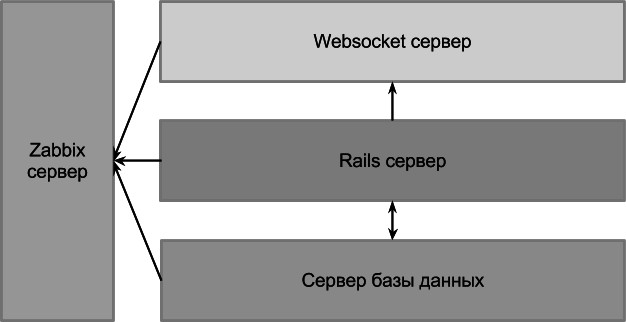
\includegraphics[width=1\linewidth]{hardware_configuration.eps}}
\caption{Схема связи между серверами}
\label{ris:hardware_configuration}
\end{figure}

На рисунке \ref{ris:hardware_configuration} изображена минимально рекомендуемая
схема серверов. При такой схеме кажный сервер выполняет свою задачу независимо
от других серверов:
\begin{enumerate}
  \item Websocket сервер обслуживает обмен сообщений между пользователями;
  \item Rails сервер обеспечивает работу непосредственно системы;
  \item Сервер базы данных обслуживает работу Postgresql базы;
  \item Zabbix сервер занимается мониторингом работы всех серверов.
\end{enumerate}

\subsection{Развертывание сайта}
Их схемы развертывания (рис. \ref{ris:deployment_sait}) видно что развертывание - это
многоэтапный процесс в котором важна последовательность этапов. Так же важно учитывать что приложение
считается обноленным только в случае если все этапы выполнены успешно. В случае
неуспешного выполения хотя бы одного из этапов необходимо обратить все
изменения. Исходя из анных фактов вытекает важно требования для системы
развертывания - транзакционность, т.е. любое изменение должно быть обратимо.

\begin{figure}[h!]
\center{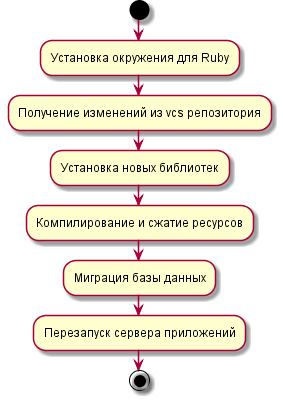
\includegraphics[width=0.5\linewidth]{deployment_sait.eps}}
\caption{Схема развертывания Ruby On Rails сайта}
\label{ris:deployment_sait}

% start
% 
% :Установка окружения для Ruby;
% :Получение изменений из vcs репозитория;
% :Установка новых библиотек;
% :Компилирование и сжатие ресурсов;
% :Миграция базы данных;
% :Перезапуск сервера приложений;
% 
% stop

\end{figure}

Для развертывания и обновления сайта на рабочем сервере существует библиотека
Capistrano. Данная библиотека позволяет настроить полностью контролируемый
процесс развертывания сайта.

Основные преимущества от использования данной библиотеки:
\begin{enumerate}
  \item поддержка транзакций и возможность обратить все изменения;
  \item гибкая настройка процесса за счет возможности выполнять любой удаленный
  \item код на сервере; 
  \item поддержка протокола ssh - необходимо для обеспечения безопасности; 
  \item интеграция с Ruby On Rails;
  \item развертывание на несколько серверов одновременно;
  \item установка окружения ruby.
\end{enumerate}

На данном этапе разработки библиотека не используется, так как нет необходимости
разворачивать приложение на рабочем сервере.

Рассмотрим инструкцию для запуска сайта в режиме разработчика.

В качестве операционой системы можно использовать любой UNIX-like дистрибутив.

Для начала нужно уставновить окружение для работы ruby, установку лучше всего
производить через rvm. Для работы проекта требуется ruby версии 1.9.3.

Далее необходимо установить базу данных Postgresql и создать пользователя в базе
данных с правами на создание баз данных. В конфигурационно файле
config/database.yml в секции development нужно выставить соответствующие логин и
пароль ждя подключения к базе данных.

Следующим шагом создадим непосредственно базу данных с помощью команды rake
db:create. База данных создана, но в ней нет необходимых таблиц. Чтобы добавить
таблицы в базу данных выполним rake db:migrate.

Для работы сайта создадим набор тестовых данных с помощью команды rake db:seed.

Запустим Websocket сервер с помощью команды rake wsserver.

Теперь можно запускать непосредственно сайт - rails s. После чего сайт будет
доступен по адресу \url{http://localhost:3000}.
\subsection{Nginx}
Архитектура работающего веб-сервера является двухуровневой. На первом уровне
находится HTTP-сервер, который перехватывает все HTTP запросы поступающие от
клиентов. В качестве такого сервера в нашем проекте используется бесплатный
сервер от Игоря Сысоева - nginx. Данный сервер длительное время он обслуживает
серверы многих высоконагруженных российских сайтов, таких как Яндекс, Mail.Ru,
ВКонтакте и Рамблер. Согласно статистике Netcraft nginx обслуживал или
проксировал 13.54\% самых нагруженных сайтов в мае 2013 года\footnote{
	\url{http://news.netcraft.com/archives/2013/05/03/may-2013-web-server-survey.html}
}.

Настройка сервера начинается с его установки. Это можно сделать обычными для
*nix систем способами - установить его через репозиторий пакетов, либо
скомпилировать из исходников с учетом особенностей конкретной рабочей машины.

Далее необходимо настроить конфигурацию для конкретного сайта (nginx позволяет
хостить множество сайтов). Для это в папке конфигурации надо создать файл с
именем сайта, как правило он расположен в папке
/etc/nginx/enabled-sites/site\_name.conf. В данном файле необходимо указать
полный URL сайта и номер порта. Также надо указать директорию в которой хранится
сайт. Как правило  для Ruby on Rails это /srv/site\_name/public.

С сервером второго уровня nginx связывается с помощью IPC-сокета, путь к 
которому указываются в конфигурационном файле сайта.
\subsection{Unicorn}
Сервер второго уровня получает поступающие запросы от сервера первого уровня,
выполняет их в среде Ruby on Rails, результат вычислений отдает в виде
стандартных веб-файлов (css, html, js) назад серверу первого уровня, который
отдает  их уже клиенту.

В качестве сервера второго уровня нами был выбран Unicorn. Данный сервер был
выбран за его популярность среди Ruby on Rails - разработчиков, что означает
наличие большого количества примеров файлов конфигурации, что ускоряет и
облегчает процесс развертывания.

Двухуровневая архитектура предоставляет возможность горизонтального
масштабирования системы. Например можно организовать кластер из серверов второго
уровня и распределять нагрузку между ними с помощью сервера первого уровня.

\subsection{Логи}
Аппаратная конфигурация системы предусматривает наличие нескольких физических
серверов. Для обеспечения дополнительного контроля за ними необходимо настроить
систему централизованного сбора логов. Данный подход позволит ускорить процесс
анализа логов за счет более удобного доступа или за счет использования утилит
для автоматического анализа логов.

\section{Бэкап}
Для обеспечения сохранности данных в системе важно создавать резервные копии
базы данных.

Существует множество решений для выполнения данной задачи. В системе
предполагается использовать решение для создания резервных копий на уровней
файловой системы - Bacula. Bacula достаточно проста в настройке и позволяет
создать распределенную систему для бэкапов.

В связке с Postgresql, Bacula позволяет создать PITR (point-in-time recovery)
бэкап - это механизм создания резервных копий, основанный на возможности
Postgresql создавать WAL-логи. WAL (Write Ahead Log) - это бинарные логи все
транзакций и запросов выполненных в базе данных. При верной настройке бэкап
будет отставать от основной базы всего на несколько минут.
\subsection{Администрирование}
При большом количестве независимых серверов возникает проблема контроля их
работы. Для обеспечения бесперебойной работы системы важно максимально быстро
выявлять проблемы в работе серверов и устранять эти проблемы.
	
Проблемы в работе серверов могут быть связаны с:
\begin{enumerate}
  \item низкой производительностью отдельных компонентов сервера (дисков, процессора);
  \item неправильной настройкой программного обеспечения или операционной
системы; 
  \item отказом оборудования;
  \item внешними факторами.
\end{enumerate}

Решение данной проблемы является настройка системы мониторинга, которая сможет
контролировать работу серверов и оповещать ответственного в случае неполадок.	

\subsubsection{Zabbix}
Zabbix\footnote{
	\url{http://www.zabbix.com/ru/}
} - это комплексное решение для мониторинга серверов различного типа,
включающее в себя:
\begin{enumerate}
  \item zabbix-agent - сервис устанавливаемый непосредственно на контролируемом сервере, позволяющий получать различные метрики работы сервера;
  \item zabbix-server - сервер собирает информацию с zabbix-agent’ов и сохраняет
ее в базу данных; сервер также занимается анализом поступающих данных и оповещает ответственных в случае если требуется вмешательство; 
  \item web интерфейс - позволяет производить настройку zabbix-server’а и
просматривать поступающие от серверов данные.
\end{enumerate}
\newpage
\chapter{Информационная безопасность}
Существует определенный набор ГОСТ’ов, подробно описывающих источники угроз и
механизмы защиты от них. В данном разделе будет рассмотрена более простая
терминогория. Большее внимание будет уделено конкретным рекомендация по
обеспечению информационной бесзопасности в разрабатываемой системе.

\section{Основные угрозы}
Предже чем приступать к составлению рекомендаций нужно определиться с
терминологией.

Угрозой будем считать процесс, результатом которого является предоставление
несанкцианированного доступа к какой-либо информации.

Человека, объект или ПО целью которого является получение доступа к зашищенной
информации будем считать злоумышленником.

Будем рассматривать следующие виды угроз информационной безопасности:

\begin{enumerate}
  \item Первая – это аппаратные средства. Сбой в работе или выход из строя процессора, материнской платы, линий связи, периферийных устройств может привести к частичной или полной потери информации, хранящейся в компьютере.
  \item Второй источник угрозы – программное обеспечение. Угрозу могут
представлять исходные и приобретенные программы, утилиты и операционные системы. Для обеспечения сохранности информации штатным пользователям рекомендуется устанавливать лицензионные антивирусные программы.
  \item Третий вид угрозы информационной безопасности – данные, которые хранятся
на отдельных носителях или в печатном виде. Необходимо принимать отдельные меры по хранению данных, которые не находятся в компьютерной системе.
  \item Четвертый вид угрозы – пользователи компьютеров и обслуживающий
персонал. Люди могут нанести вред информации как случайно, так и специально. Поэтому всегда количество людей, имеющих доступ к информации организации, сведен до минимума. Большинство организаций открывают в штате должность специалиста по информационной безопасности, который отвечает за сохранность данных компьютерных систем.
\end{enumerate}

\section{Обеспечение безопасности}
\subsection{Аппаратный уровень}
Прежде всего нужно предотвращать физический доступ к серверам на которых
расположена важная информаци. В контексте разработанной системы - это любой
физический сервер непосредственно обеспечивающий работоспособность системы.

Так же важно резервировать основные компоненты системы и производить постоянное
архивирование важных данных для предотвращения потерь в случае сбоя в
оборудовании.

Давать более конкретные рекомендации для данного уровня не имеет смысла, так как
по большей части все зависит от конкретной схемы установки системы.

\subsection{Программный уровень}
На данном уровне обеспечение безопасности необходимо как на уровне
разрабатываемой системы, так и на уровне операционной системы и на уровне
обслуживающего програмного обеспечения.

Важно устанавливать програмное обеспечение только из доверенных источников;

На каждом физическом узле системы обеспечивать связь с другими узлами на
минимальном необходимом уровне. Прежде всего это значит закрытие все
неиспользуемых при работе системы портов. Конфигурация используемы портов
зависит от расположения компонентов системы и настроек системы. По-умолчанию в
системе используются следующие порты:
\begin{enumerate}
  \item 80 - Nginx;
  \item 5432 - Postgresql;
  \item 22 - ssh;
  \item 25 - SMTP;
  \item 8081 - Websocket server.   
\end{enumerate}

При использовании дополнительного программного обеспечения (бэкапы, логи) могут
использоваться:
\begin{enumerate}
  \item 9101, 9102, 9103 - Bacula;
  \item 514 - syslog.   
\end{enumerate}

Доступ к серверам по протоколу ssh должен быть разрешен только с компьютеров
ответственных лиц.

На каждом сервере должно быть настроено логирование всех действий, для
расследования сбоев системы и случаев несанкционированного доступа.

Любые кофигурационные файлы и настройки системы не должны располагаться в
публичном доступе.

По возможности необходимо обеспечить использование SSL протокола для доступа к
серверу приложений.

Для развертывания системы нужны права ни модификацию и изменение схемы базы
данных. Необходимо забирать данные привилегии после установки для предотвращения
несанкцианированного изменения схемы базы данных.

\subsection{Человеческий фактор}
Частично на уровне системы реализована защита от человеческого фактора. В
частности при длительном бездействии авторизованного пользователя будет
произведена блокировка аккаунта. Так же система предоставляет доступ
авторизованному пользователю только к определенной информации.

\subsection{Политика информационной безопасности}
Принятие ПИБ важный этап при организации безопасности системы. Политика должна
быть разработа соответствующим отделом или руководством предприятия с целью
повышения уровня защищенности информации.

\newpage
\section*{Выводы}
\addcontentsline{toc}{section}{Выводы}
Основная цель исследований представленных в данной ипломной работе заключалась в
создании системы мониторинга состояния детей в врожденным пороком сердца.
Базой для исследований стала деятельность Кузбасского кардиологического центра.
Были формализованны текущие бизнес-процессы и выявлены проблемы их
функционирования. Основной проблемой оказалась невозможность постоянного
наблюдения за состоянием пациента.

На основе проблем были сформированы цели. Основной целью стала организация
постоянного мониторинга состояния пациента. 

Для достижения цели были составлены требования к будущей системе. Основным требования стало
создание технической базы, которая позволяла бы получать диагностические данные
от пациента в максимально удобной для пациента форме. Так же важной технической
возможностью системы является получение диагностических данных с медицинских
устройств.

На основе целей были сформированы требования к будущей системе. Требования
включают в себя как набор необходимых функциональных возможностей системы, так и
требования к технической реализации.

Ни одно готовое решение не подошло под составленные требования. Основными
причинами были: спорная техническая реализация, отсутствие части функционала,
высокая стоимость. Именно после этого шага было принято разрабатывать
собственную систему.

На начальном этапе разработки были скорректированны существующие
бизнес-процессы, для адаптации их к новым требованиям. Далее была спроектирована
основная архитектура системы. Было решено реализовывать всю функциональность на
основе web-технологий. Основной причиной стала высокая доступность и
распространенность этих технологий.

Основную сложность при разработке новой системы создал вопрос с выбором
конкретных технологий. Были рассмотрены и испробованы различные технические
решения. В итоге выбор был сделан в пользу Ruby On Rails, как решения
предоставляющего наилучшую инраструктуру для разработки.

После продолжительного этапа разработки была реализована основная архитектура
системы и функциональность. Однако на данном этапе система еще непригодна для
использования на реальном предприятии.

Исходный код текущей реализации доступен в публичном репозитории
(\url{https://github.com/crashr42/shm}).

\newpage
\section*{Словарь терминов и определений}
\addcontentsline{toc}{section}{Словарь терминов и определений}
\underline{Развертывание} - процесс переноса приложения на рабочий сервер и
последующий запуск приложения в рабочем режиме.

\underline{Issue tracking} - программное обеспечение для создания задач с
возможностями:
\begin{enumerate}
  \item отслеживать статус выполнения задач;
  \item комментировать задачи;
  \item соотносить изменения в коде с задачей.
\end{enumerate}

\underline{MVC} («Модель-представление-контроллер») - схема использования
нескольких шаблонов проектирования, с помощью которых модель данных приложения,
пользовательский интерфейс и взаимодействие с пользователем разделены на три
отдельных компонента так, что модификация одного из компонентов оказывает
минимальное воздействие на остальные.  Каждый из компонентов означает:
\begin{enumerate}
  \item Модель - предоставляет знания: данные и методы работы с этими данными, реагирует на запросы, изменяя своё состояние. Не содержит информации, как эти знания можно визуализировать.
  \item Представление, вид - отвечает за отображение информации (визуализацию).
Часто в качестве представления выступает форма (окно) с графическими элементами.
  \item Контроллер - обеспечивает связь между пользователем и системой:
контролирует ввод данных пользователем и использует модель и представление для реализации необходимой реакции.   
\end{enumerate}

\underline{ORM} (Object-relational mapping) - технология программирования,
которая связывает базы данных с концепциями объектно-ориентированных языков
программирования, создавая «виртуальную объектную базу данных».

\underline{REST} (Representational State Transfer) - «передача представлений
состояний».
Был предложен в 2000 году Роем Филдингом. Данные в REST должны передаваться в
виде небольшого количества стандартных форматов (например HTML, XML, JSON).
Сетевой протокол (как и HTTP) должен поддерживать кэширование, не должен
зависеть от сетевого слоя, не должен сохранять информацию о состоянии между
парами «запрос-ответ».

\underline{HTTP} (HyperText Transfer Protocol) -  протокол прикладного уровня
передачи данных (изначально — в виде гипертекстовых документов). Основой HTTP является
технология «клиент-сервер», то есть предполагается существование потребителей
(клиентов), которые инициируют соединение и посылают запрос, и поставщиков
(серверов), которые ожидают соединения для получения запроса, производят
необходимые действия и возвращают обратно сообщение с результатом.

\underline{XML} (eXtensible Markup Language) - рекомендованный Консорциумом
Всемирной паутины (W3C) язык разметки. Спецификация XML описывает XML-документы и частично
описывает поведение XML-процессоров (программ, читающих XML-документы и
обеспечивающих доступ к их содержимому). XML разрабатывался как язык с простым
формальным синтаксисом, удобный для создания и обработки документов программами
и одновременно удобный для чтения и создания документов человеком, с
подчёркиванием нацеленности на использование в Интернете. Язык называется
расширяемым, поскольку он не фиксирует разметку, используемую в документах:
разработчик волен создать разметку в соответствии с потребностями к конкретной
области, будучи ограниченным лишь синтаксическими правилами языка. Сочетание
простого формального синтаксиса, удобства для человека, расширяемости, а также
базирование на кодировках Юникод для представления содержания документов привело
к широкому использованию как собственно XML, так и множества производных
специализированных языков на базе XML в самых разнообразных программных
средствах.

\underline{JSON} (JavaScript Object Notation) - текстовый формат обмена данными,
основанный на JavaScript и обычно используемый именно с этим языком. Как и
многие другие текстовые форматы, JSON легко читается людьми.

\underline{HTML} (HyperText Markup Language) - стандартный язык разметки
документов во Всемирной паутине. Большинство веб-страниц создаются при помощи
языка HTML (или XHTML). Язык HTML интерпретируется браузерами и отображается в
виде документа в удобной для человека форме. HTML является приложением («частным
случаем») SGML (стандартного обобщённого языка разметки) и соответствует
международному стандарту ISO 8879. XHTML же является приложением XML.

\underline{CRUD} (Create Read Update Delete) - сокращённое именование 4 базовых
функций при работе с персистентными хранилищами данных — создание, чтение,
редактирование и удаление.

\underline{DDL} (Data Definition Language) - это семейство компьютерных языков,
используемых в компьютерных программах для описания структуры баз данных.

\underline{Websocket} - протокол полнодуплексной связи поверх TCP-соединения,
предназначенный для обмена сообщениями между браузером и веб-сервером в режиме
реального времени.

\underline{Hot Standby} - механизм поддержки состояния резервного компонента
системы в актуальном состоянии, позволяющий производить замену основного
компонента без задержки.

\underline{SMTP} (Simple Mail Transfer Protocol — простой протокол передачи
почты) — это сетевой протокол, предназначенный для передачи электронной почты в
сетях TCP/IP.

\underline{SSH} (Secure SHell) - сетевой протокол прикладного уровня,
позволяющий производить удалённое управление операционной системой и
туннелирование TCP-соединений (например, для передачи файлов). Схож по
функциональности с протоколами Telnet и rlogin, но, в отличие от них, шифрует
весь трафик, включая и передаваемые пароли. SSH допускает выбор различных
алгоритмов шифрования. SSH-клиенты и SSH-серверы доступны для большинства
сетевых операционных систем.

\underline{Unix domain socket} (Доменный сокет Unix) или IPC-сокет (сокет
межпроцессного взаимодействия) — конечная точка обмена данными, схожая с
Интернет-сокетом, но не использующая сетевой протокол для взаимодействия (обмена
данными). Он используется в операционных системах, поддерживающих стандарт
POSIX, для межпроцессного взаимодействия. Корректным термином стандарта POSIX
является POSIX Local IPC Sockets.

\underline{SSL} (Secure Sockets Layer) - криптографический протокол, который
обеспечивает безопасность связи через Интернет. Он использует асимметричную
криптографию для аутентификации ключей обмена, симметричное шифрование для
сохранения конфиденциальности, а коды аутентификации сообщений для целостности
сообщений.

\nocite{*}
\newpage
\bibliographystyle{ugost2008ls}
\bibliography{biblio}
\ESKDappendix{справочное}{Существующие бизнес-процессы\label{app:asis}}

\begin{figure}[h]
\center{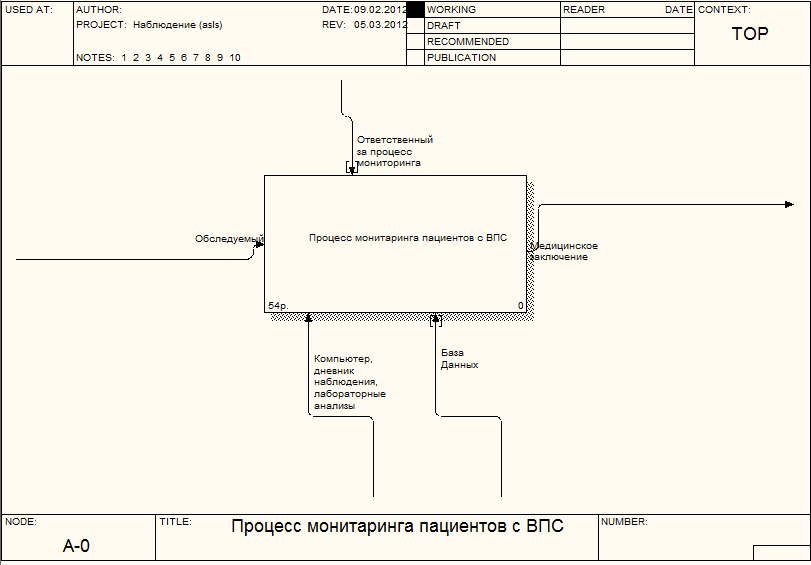
\includegraphics[width=1\linewidth,angle=90]{before_decomposition.eps}}
\caption{Общая схема процесса мониторинга}
\label{app:before_decomposition}
\end{figure}

\newpage \begin{figure}[h]
\center{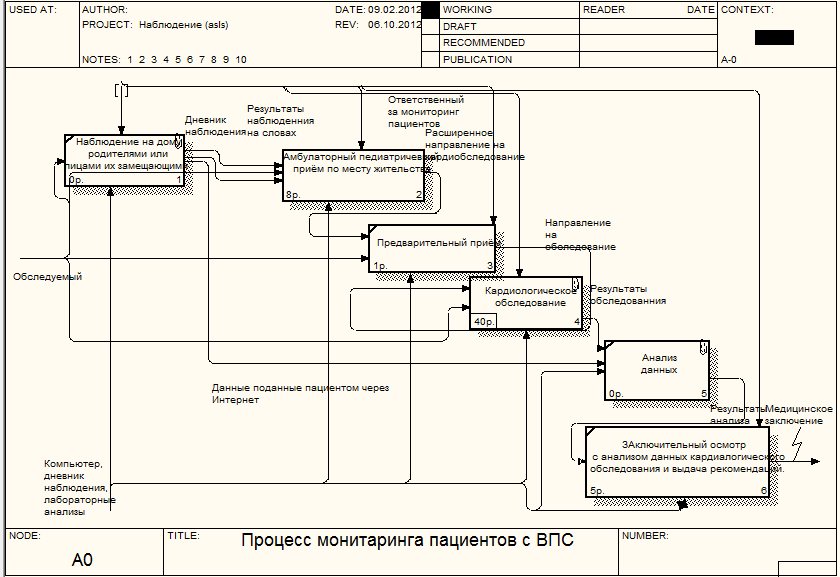
\includegraphics[width=1\linewidth,angle=90,
scale=1.2]{as_is_general_diagram.eps}}
\caption{Декомпозиция процесса мониторинга}
\label{app:as_is_general_diagram}
\end{figure}

\newpage \begin{figure}[h] \center{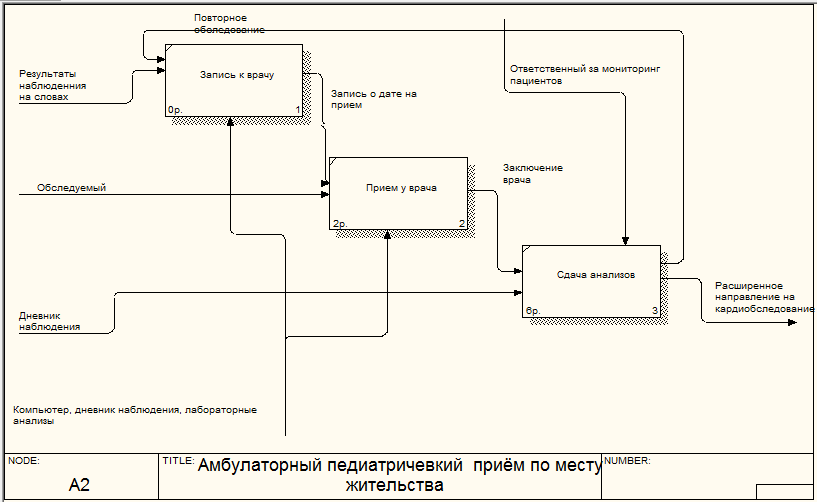
\includegraphics[width=1\linewidth,angle=90,
scale=1.2]{ambulator_appointment.eps}}
\caption{Прием у врача}
\label{app:ambulator_appointment}
\end{figure}
% \ESKDappendix{справочное}{Тестирование событий\label{app:events_tests}}

\begin{lstlisting}[language=Ruby] 
require 'spec_helper'

T = Class.new(Event) do
  child_events :event, :predicted_time => 15.minutes
end

describe Event do
  it 'default status for event - free' do
    e = create(:event)
    e.status.should eq(:free)
  end

  # #{Проверяем что события с всеми возможными статусами - являются валидными}
  context 'should be valid' do
    %w(free busy process close).each do |s|
      it "#{s} event" do
        e = create("#{s}_event".to_sym)
        e.should be_valid
      end
    end
  end

  # #{Если продолжительность события сбрасывается на 0 ->}
  # #{статус события должен изменится на busy} 
  # #{при этом статус события не меняется явным образом}
  it 'change status to busy if duration change to 0' do
    e = create(:free_event)
    e.status.should eq(:free)
    e.duration.should_not eq(0)
    e.duration = 0
    e.save!
    e.status.should eq(:busy)
  end

  # #{Если событие меняет статус с busy на free ->}
  # #{продолжительность события вычилсяется как разница в секундах} 
  # #{между датой окончания и датой начала события}
   it 'change duration to equal difference between date_end
    and date_start if status change from busy to free' do
    e = create(:busy_event)
    e.status.should eq(:busy)
    e.duration.should eq(0)
    e.status = :free
    e.save!
    e.status.should eq(:free)
    e.duration.should eq((e.date_end - e.date_start).to_i)
  end

  # #{Если продолжительность события выставляется больше 0} 
  # #{и статус события равен busy ->} 
  # #{статус события меняется на free}
  it 'change status to free if duration set greater than 0' do
    e = create(:busy_event)
    e.duration = 2
    e.save!
    e.duration.should eq(2)
    e.status.should eq(:free)
  end

  # #{Изменение статуса приоритетнее чем изменение продолжительности события}
  it 'change in the status of priority than change duration' do
    e = create(:free_event)
    e.duration = 2
    e.status = :busy
    e.save!
    e.duration.should eq(0)
    e.status.should eq(:busy)
  end

  # #{Для новой сущности продолжительность вычисляется автоматически как} 
  # #{разница между датой начала и датой окончания события}
  it 'calculate duration for new record' do
    e = build(:free_event)
    e.duration.should eq(nil)
    e.save!
    e.duration.should eq((e.date_end - e.date_start).to_i)
  end

  # #{Для уже сохраненной сущности продолжительность события не вычилсяется}
  it 'don\'t calculate duration for saved record' do
    e = create(:free_event)
    new_duration = (e.date_end - e.date_start).to_i + 1
    e.duration = new_duration
    e.save!
    e.duration.should eq(new_duration)
  end

  # #{Проверяем создание дочерних событий}
  it 'should create child events' do
    d = DateTime.now.at_beginning_of_hour
    e = T.new({
                  :date_start => d,
                  :date_end => d + 2.hours,
                  :description => 'some d',
                  :summary => 'some s'
              })
    e.save!
    e.events.count.should eq(8)
  end

  # #{Проверяем что}
  # #{изменени статуса для дочернего события с free на busy ->}
  # #{уменьшает продолжительность родительского события}
  # #{изменени статуса для дочернего события с busy на free ->}
  # #{увеличивает продолжительность родительского события} 
  it 'should subtract parent duration then status change from free to busy' do
    d = DateTime.now.at_beginning_of_hour
    e = T.new({
                  :date_start => d,
                  :date_end => d + 2.hours,
                  :description => 'some d',
                  :summary => 'some s'
              })
    e.save!
    ef = e.events.first

    equal_duration = e.duration - ef.duration
    ef.status = :busy
    ef.save!
    e.reload
    ef.status.should eq(:busy)
    e.duration.should eq(equal_duration)

    equal_duration = e.duration + (ef.date_end - ef.date_start)
    ef.status = :free
    ef.save!
    e.reload
    e.duration.should eq(equal_duration)
  end

  # #{Проверка изменения статуса события на другие статусы}
  context 'not available change status from busy' do
    it 'to close' do
      e = create(:busy_event)
      e.status = :close
      e.should_not be_valid
    end
  end

  context 'not available change status from process' do
    [:busy, :free].each do |s|
      it "to #{s}" do
        e = create(:process_event)
        e.status = s
        e.should_not be_valid
      end
    end
  end

  context 'not available change status from close' do
    [:process, :busy, :free].each do |s|
      it "to #{s}" do
        e = create(:close_event)
        e.status = s
        e.should_not be_valid
      end
    end
  end

  context 'not available change status from free' do
    [:process, :close].each do |s|
      it "to #{s}" do
        e = create(:free_event)
        e.status = s
        e.should_not be_valid
      end
    end
  end
end
\end{lstlisting}
\ESKDappendix{справочное}{Диаграмма базы данных\label{app:database_diagram}}

\begin{figure}[h]
\center{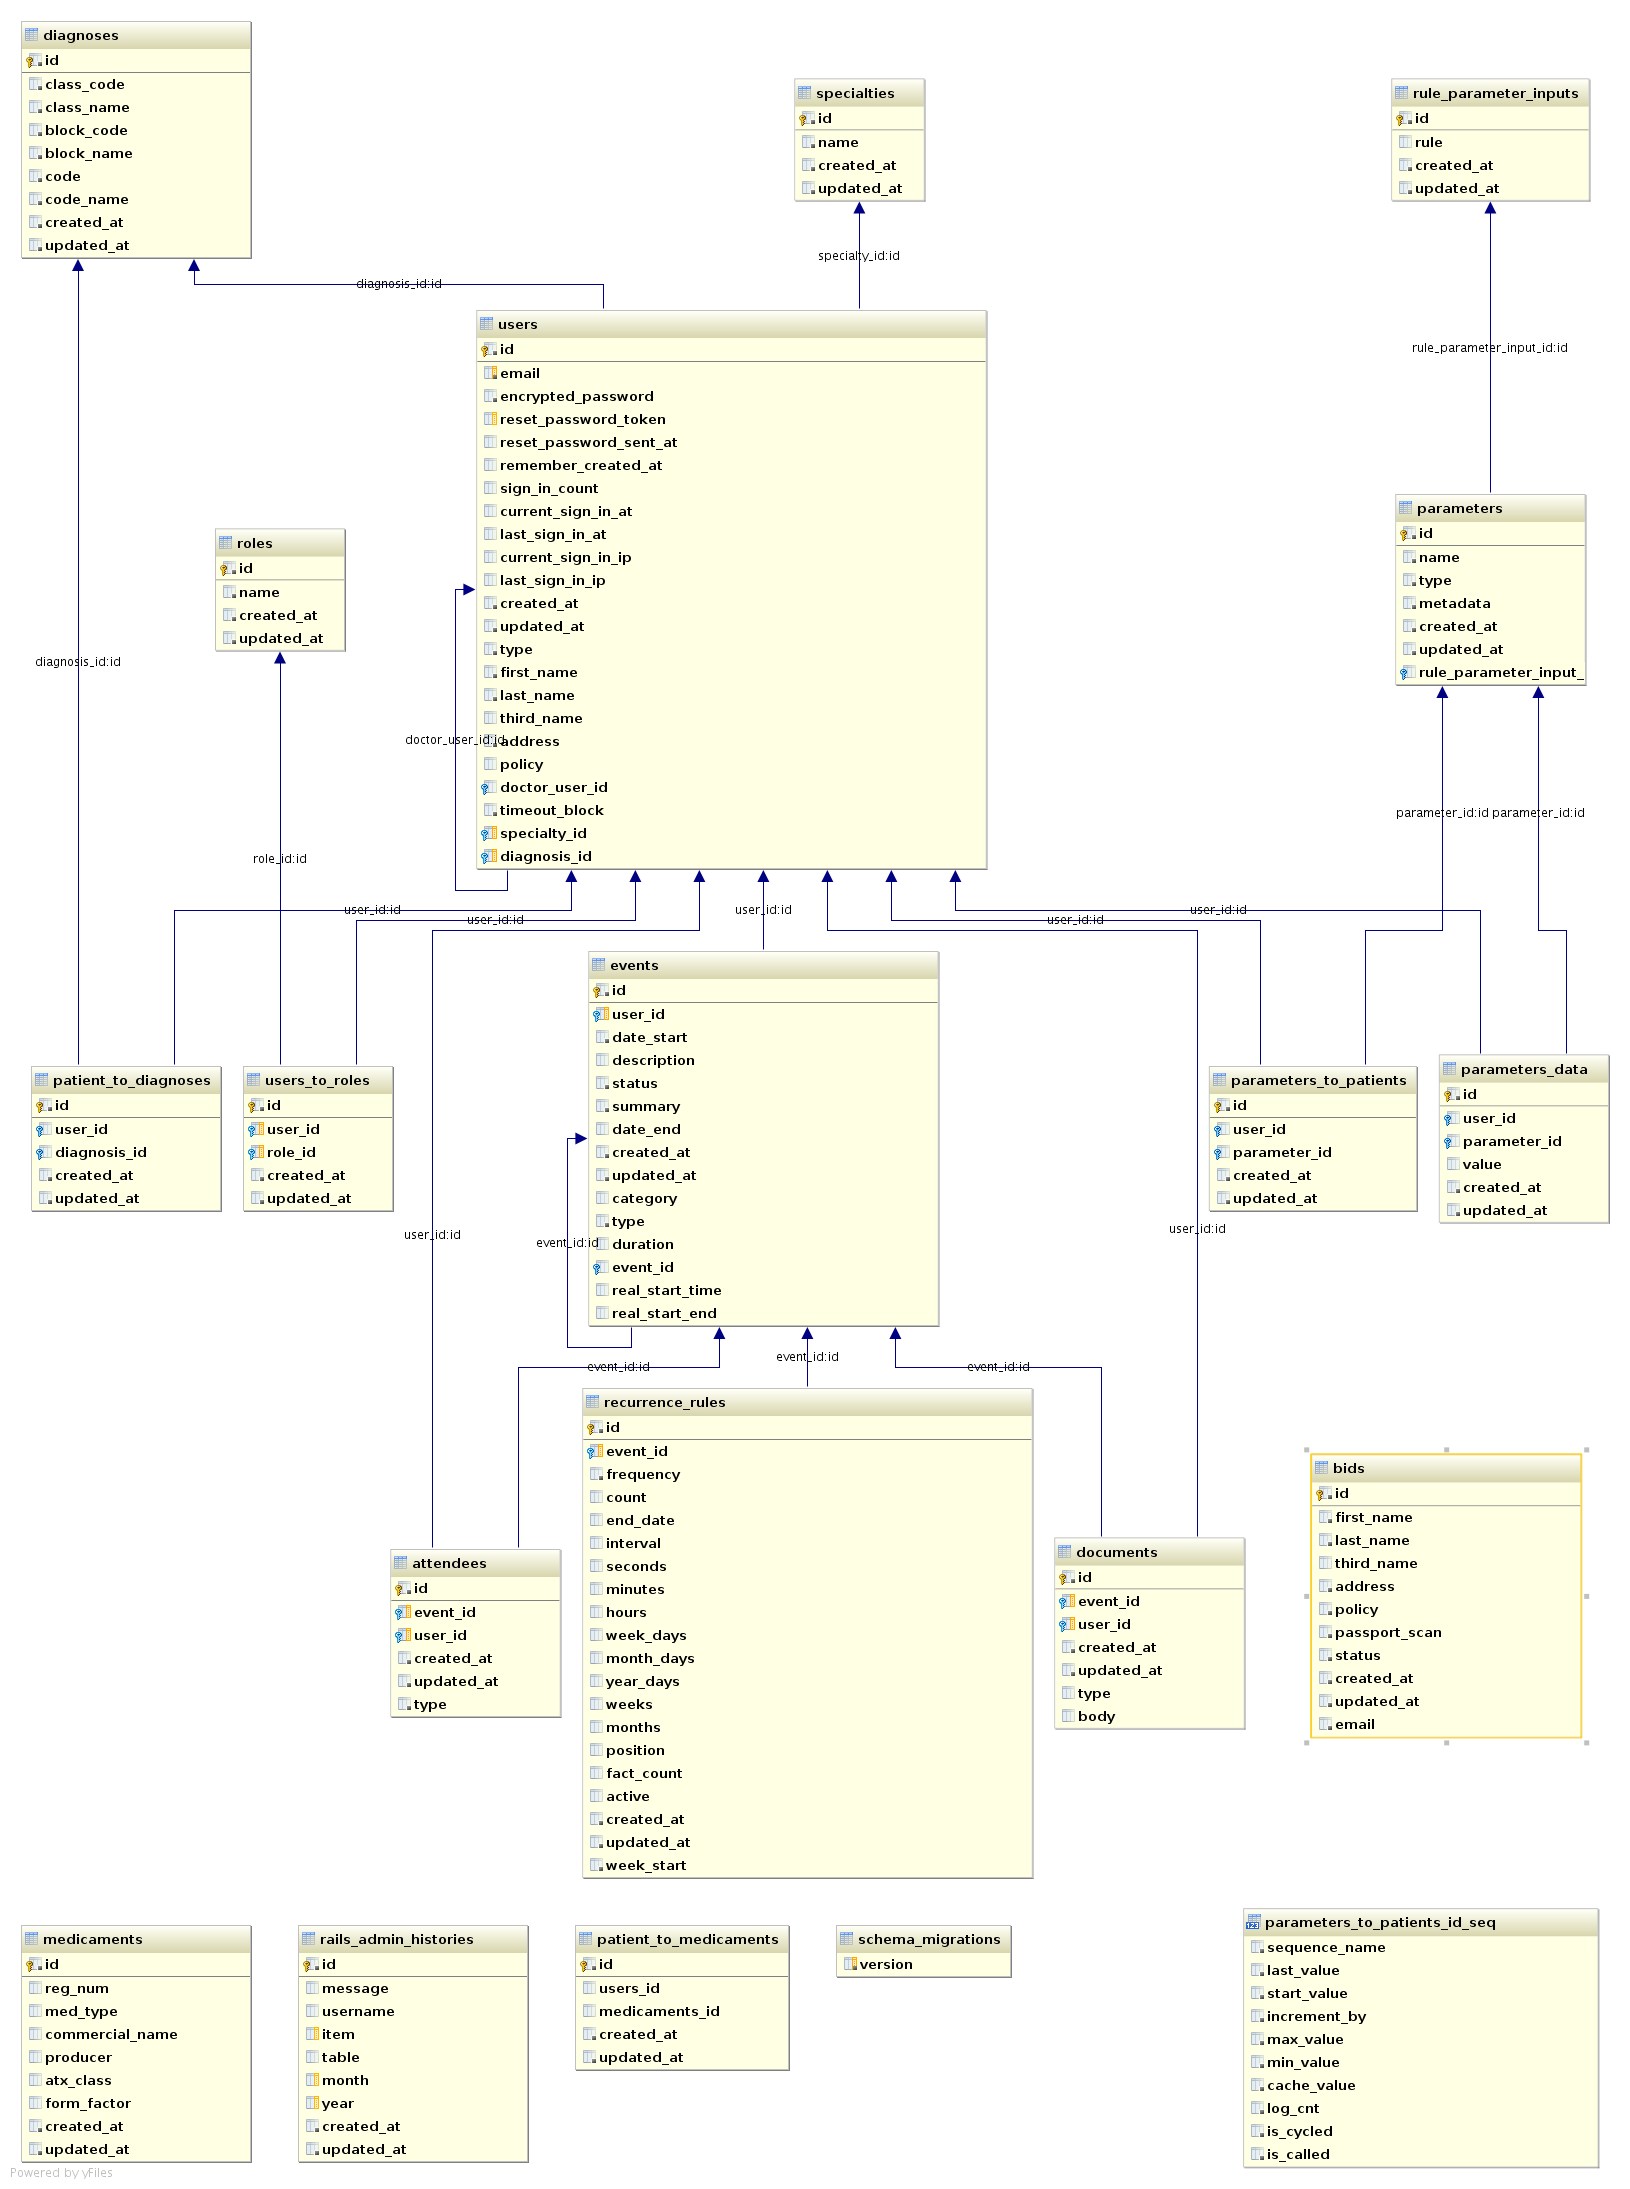
\includegraphics[width=1\linewidth,angle=90,scale=1.15]{database_diagram.eps}}
\end{figure}

\ESKDappendix{справочное}{Процесс мониторинга\label{app:tobe}}

\begin{figure}[h]
\center{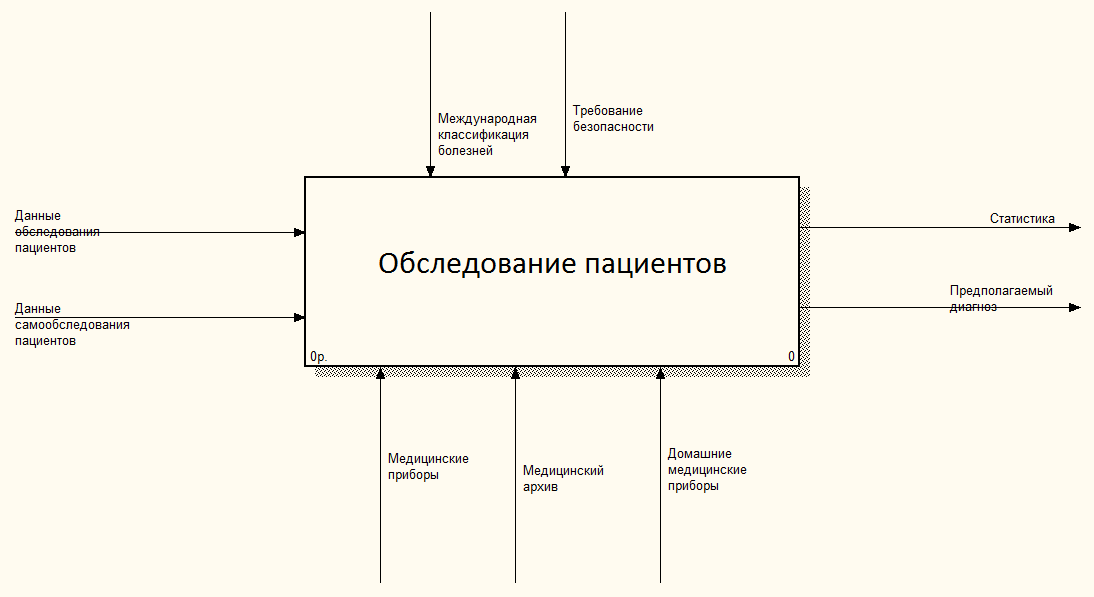
\includegraphics[width=1\linewidth,angle=90]{to_be_main_view.eps}}
\caption{Общая схема процесса мониторинга}
\label{app:tobe_main}
\end{figure}

\newpage \begin{figure}[h]
\center{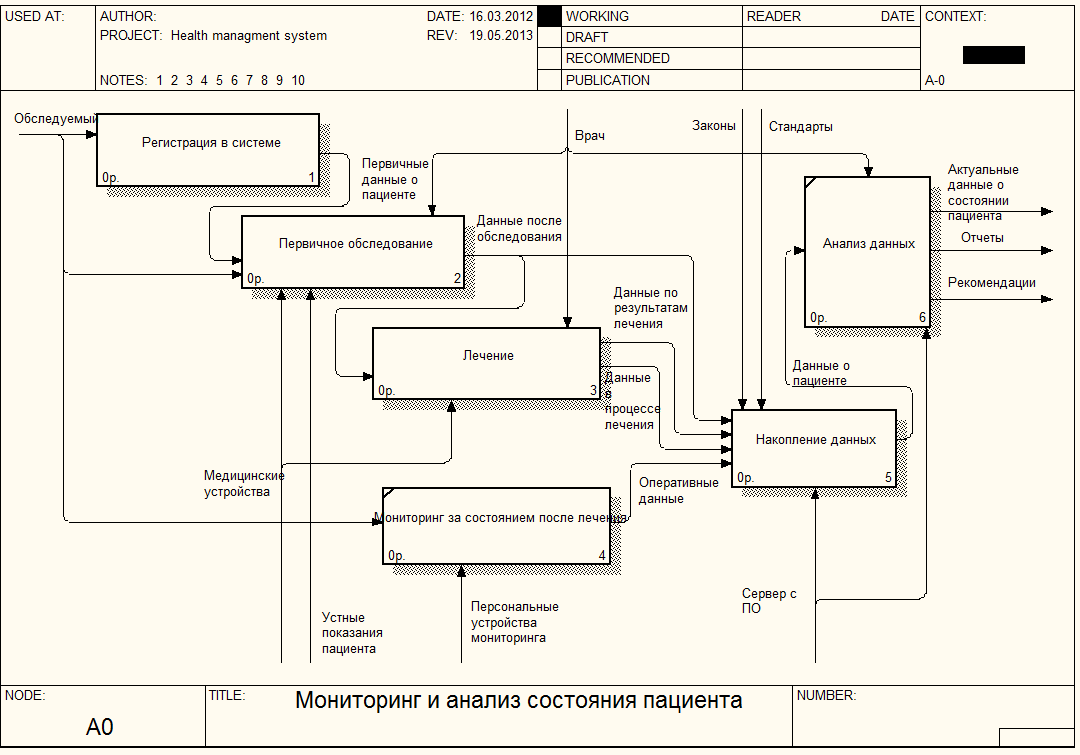
\includegraphics[width=1\linewidth,angle=90]{decomposition_to_be.eps}}
\caption{Декомпозиция процесса мониторинга}
\label{app:tobe_decomposition}
\end{figure}

\newpage \begin{figure}[h]
\center{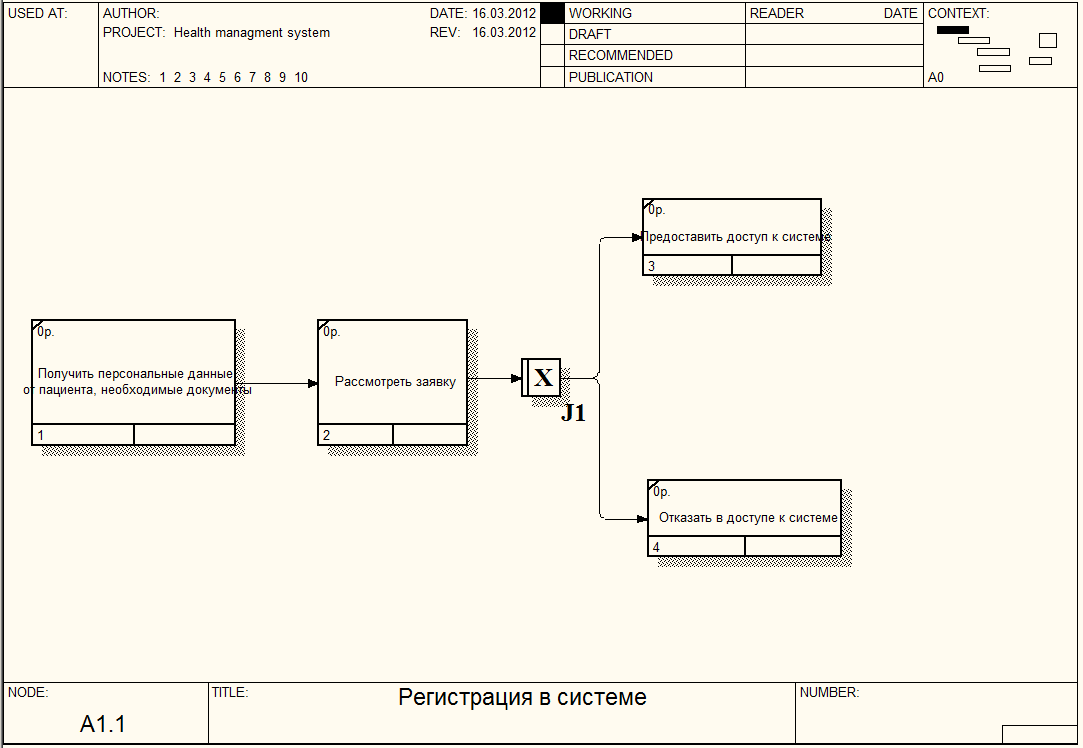
\includegraphics[width=1\linewidth,angle=90]{to_be_registration.eps}}
\caption{Регистрация в системе}
\label{app:tobe_registration}
\end{figure}

\newpage \begin{figure}[h]
\center{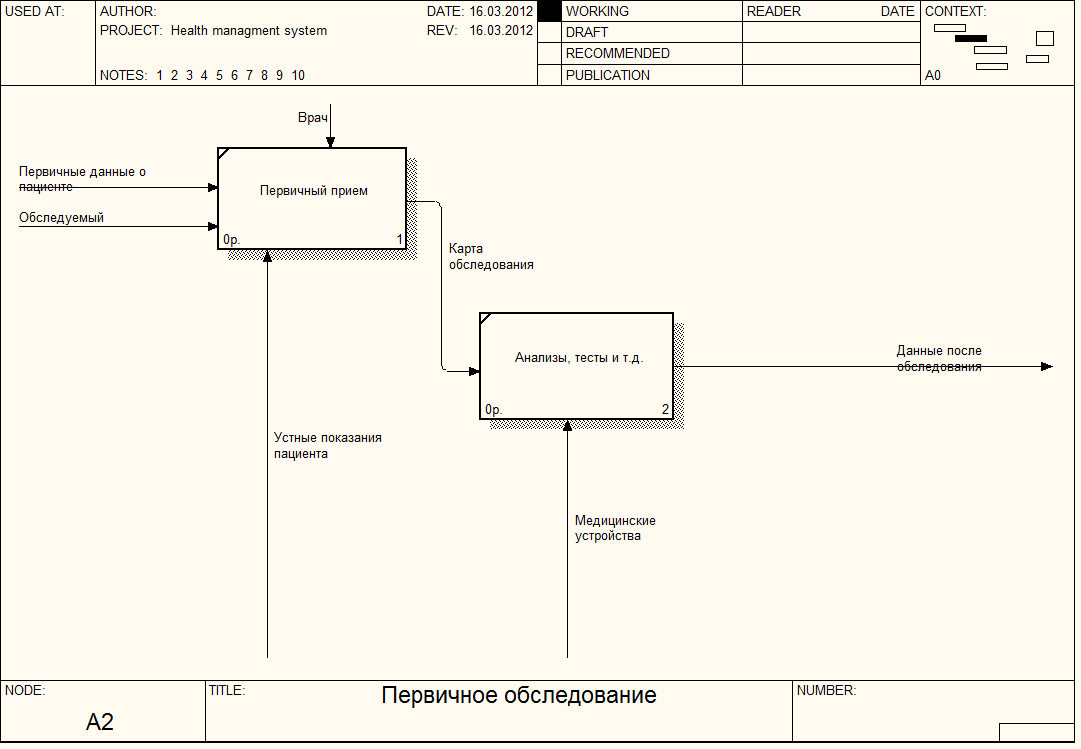
\includegraphics[width=1\linewidth,angle=90]{to_be_first_appointment.eps}}
\caption{Первичное обследование}
\label{app:tobe_first_appointment}
\end{figure}

\newpage \begin{figure}[h]
\center{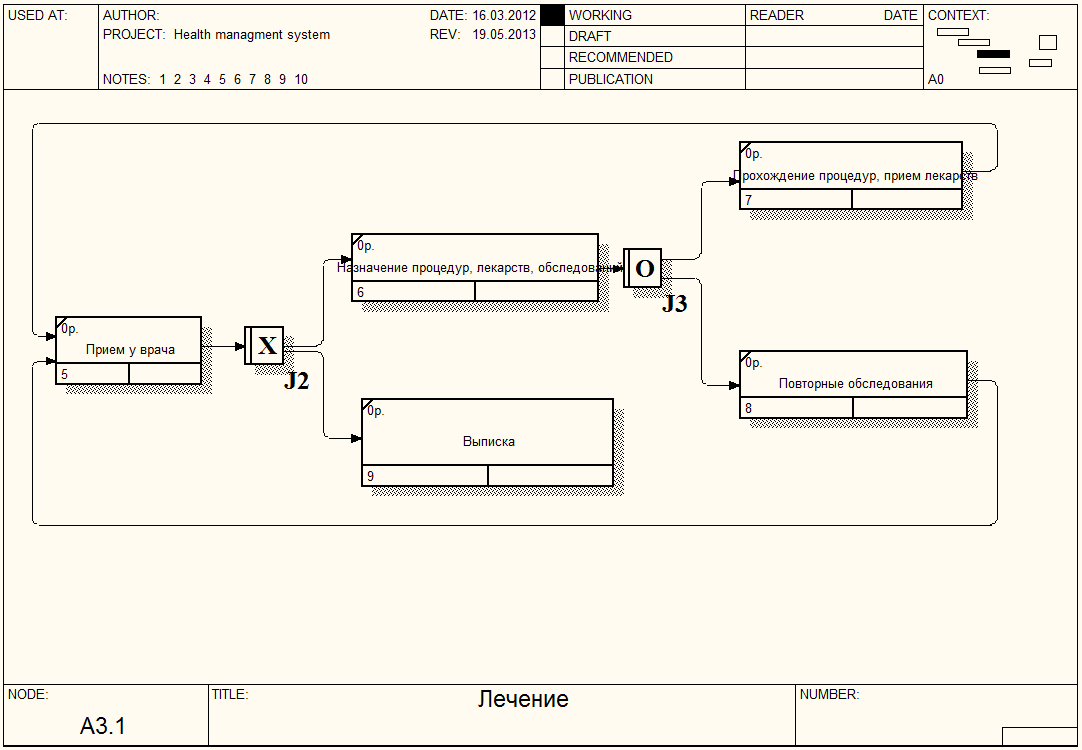
\includegraphics[width=1\linewidth,angle=90]{to_be_repaire.eps}}
\caption{Лечение}
\label{app:tobe_repaire}
\end{figure}

\newpage \begin{figure}[h]
\center{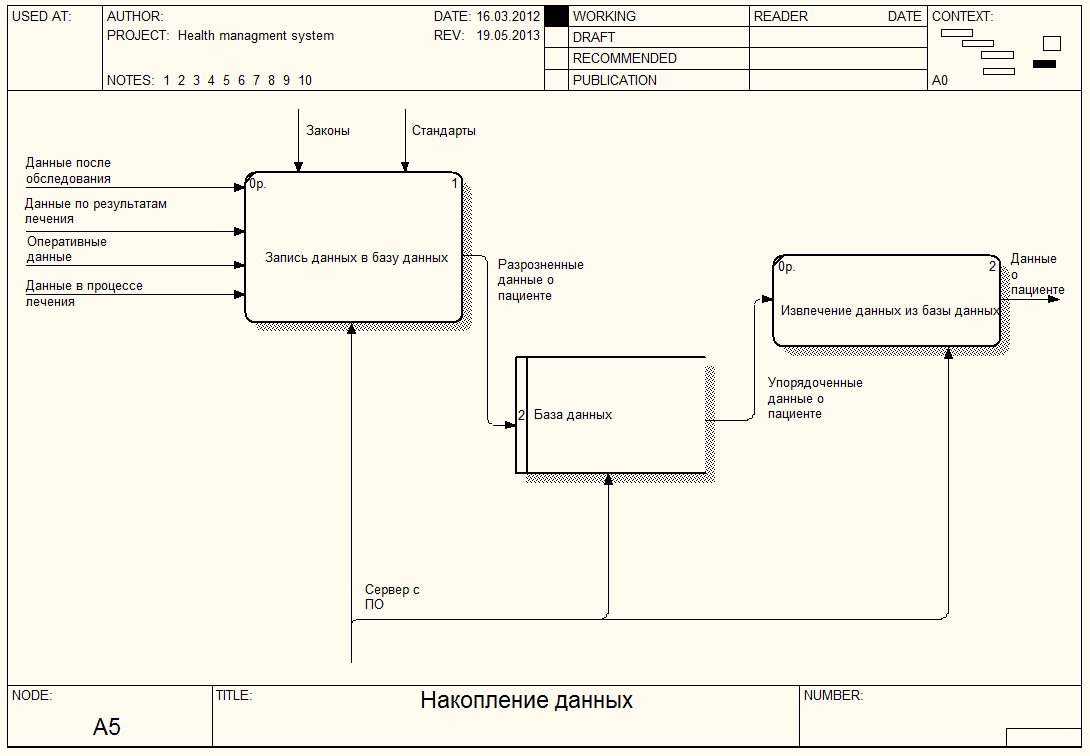
\includegraphics[width=1\linewidth,angle=90]{to_be_collect_metrics.eps}}
\caption{Накопление данных в процессе мониторинга}
\label{app:tobe_collect_metrics}
\end{figure}
\ESKDappendix{справочное}{Кабинеты\label{app:cabinets}}

\begin{figure}[h]
\center{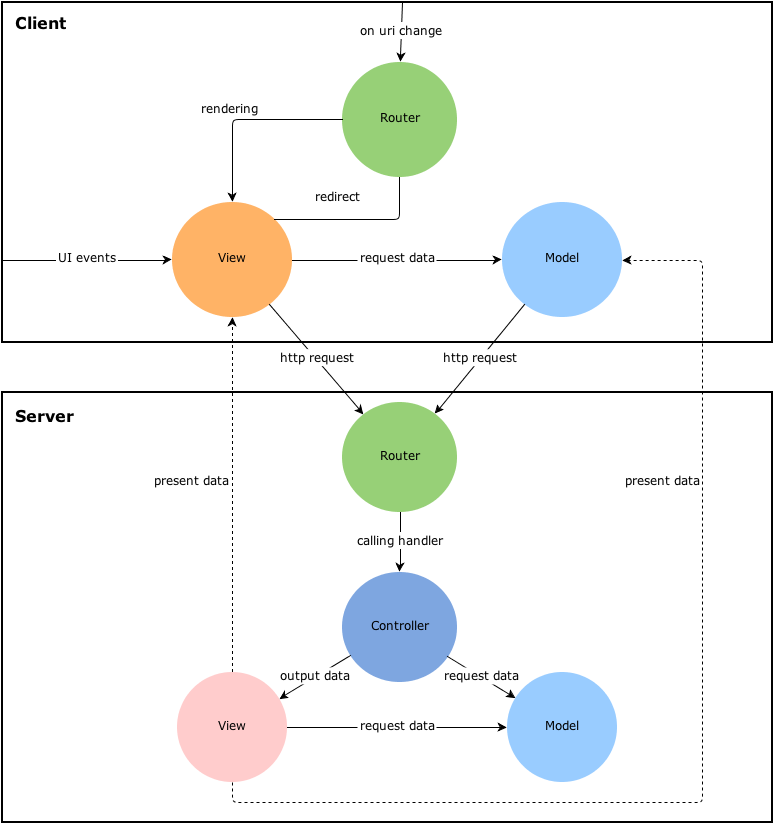
\includegraphics[width=0.9\linewidth]{cabinet_sequence.eps}}
\caption{Сценарий работы личного кабинета}
\label{app:cabinet_sequence}
\end{figure}

\newpage
\begin{figure}[h]
\center{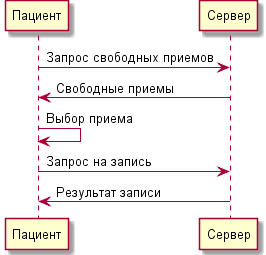
\includegraphics[width=0.6\linewidth]{patient_assigning_appointment_seq_diagr.eps}}
\caption{Кабинет доктора: сценарий записи пациента на прием}
\label{app:patient_assigning_appointment_seq_diagr}
\end{figure}

\newpage
\begin{figure}[h]
\center{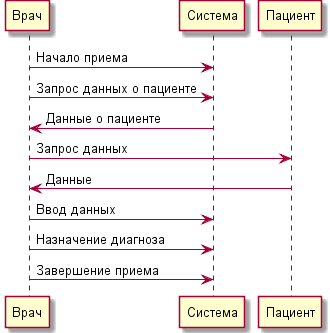
\includegraphics[width=0.6\linewidth]{doctor_cabient_appointment.eps}}
\caption{Кабинет доктора: сценарий приема пациента}
\label{app:doctor_cabient_appointment}

% Врач -> Система : Начало приема
% Врач -> Система : Запрос данных о пациенте
% Система -> Врач : Данные о пациенте
% Врач -> Пациент : Запрос данных
% Пациент -> Врач : Данные
% Врач -> Система : Ввод данных
% Врач -> Система : Назначение диагноза
% Врач -> Система : Завершение приема

\end{figure}

\newpage
\begin{figure}[h]
\center{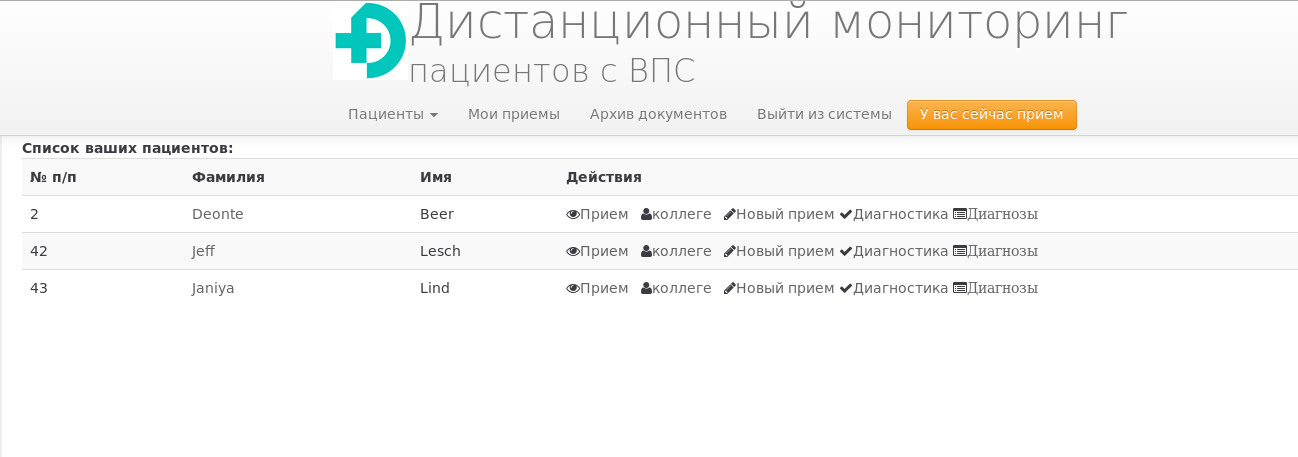
\includegraphics[width=1\linewidth,angle=90]{doctor_cabinet_patients.eps}}
\caption{Кабинет доктора: список пациентов}
\label{app:doctor_cabinet_patients}
\end{figure}

\newpage \begin{figure}[h]
\center{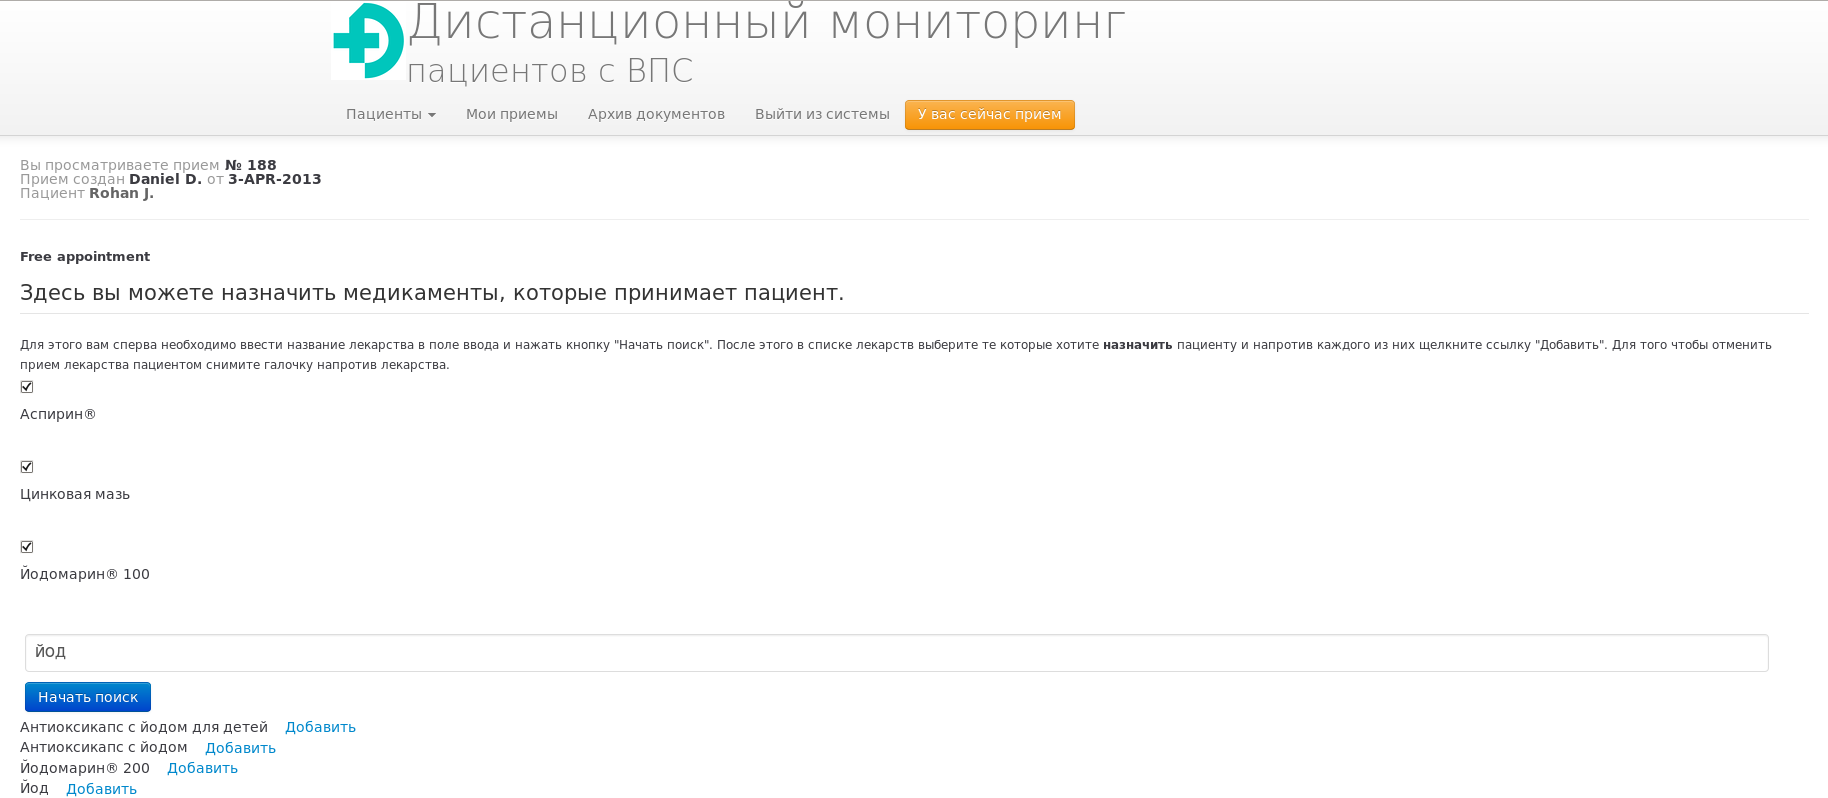
\includegraphics[width=1\linewidth,angle=90]{doctor_cabient_medicament.eps}}
\caption{Кабинет доктора: назначение лекарства}
\label{app:doctor_cabinet_medicament}
\end{figure}

\newpage \begin{figure}[h]
\center{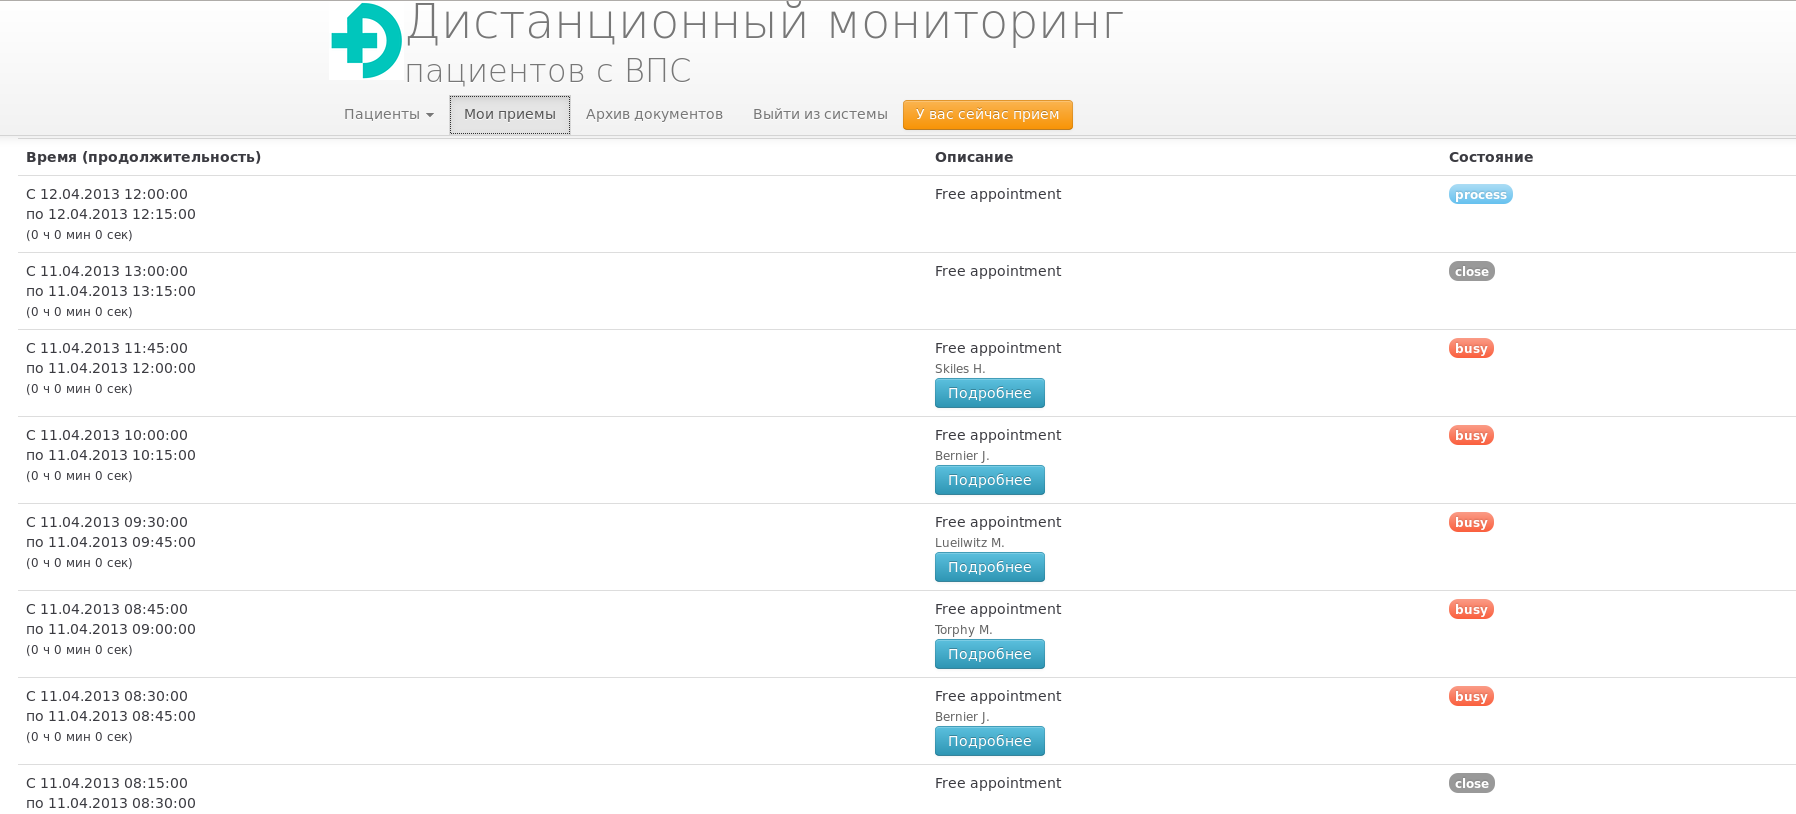
\includegraphics[width=1\linewidth,angle=90]{doctor_cabinet_appointments.eps}}
\caption{Кабинет доктора: список приемов}
\label{app:doctor_cabinet_appointments}
\end{figure}

\newpage \begin{figure}[h]
\center{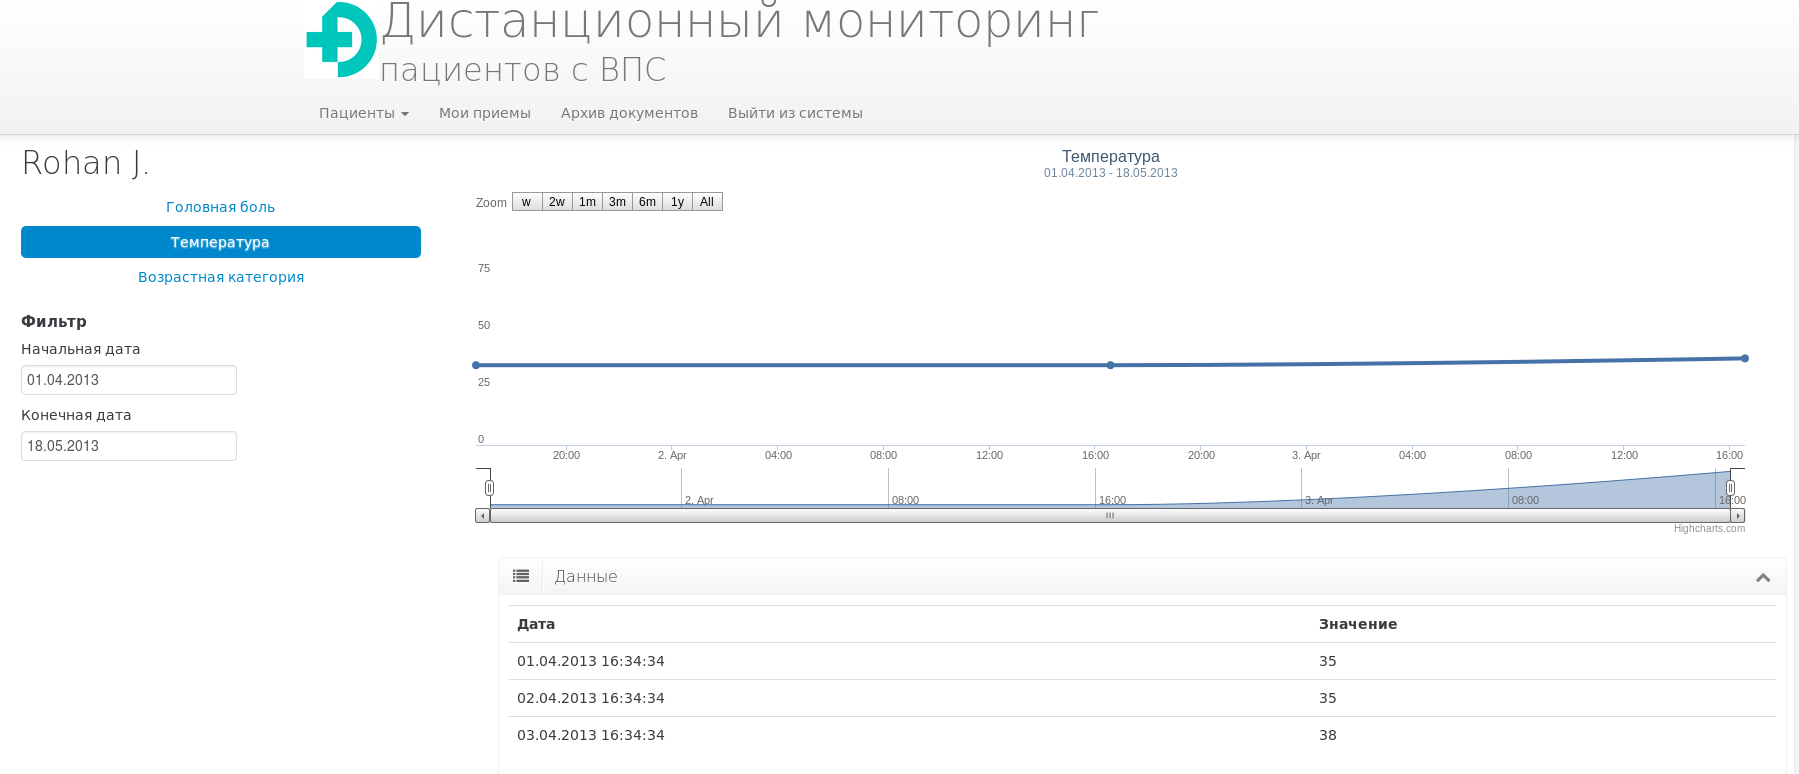
\includegraphics[width=1\linewidth,angle=90]{doctor_cabinet_diagnostic.eps}}
\caption{Кабинет доктора: диагностика}
\label{app:doctor_cabinet_diagnostic}
\end{figure}

\newpage \begin{figure}[h]
\center{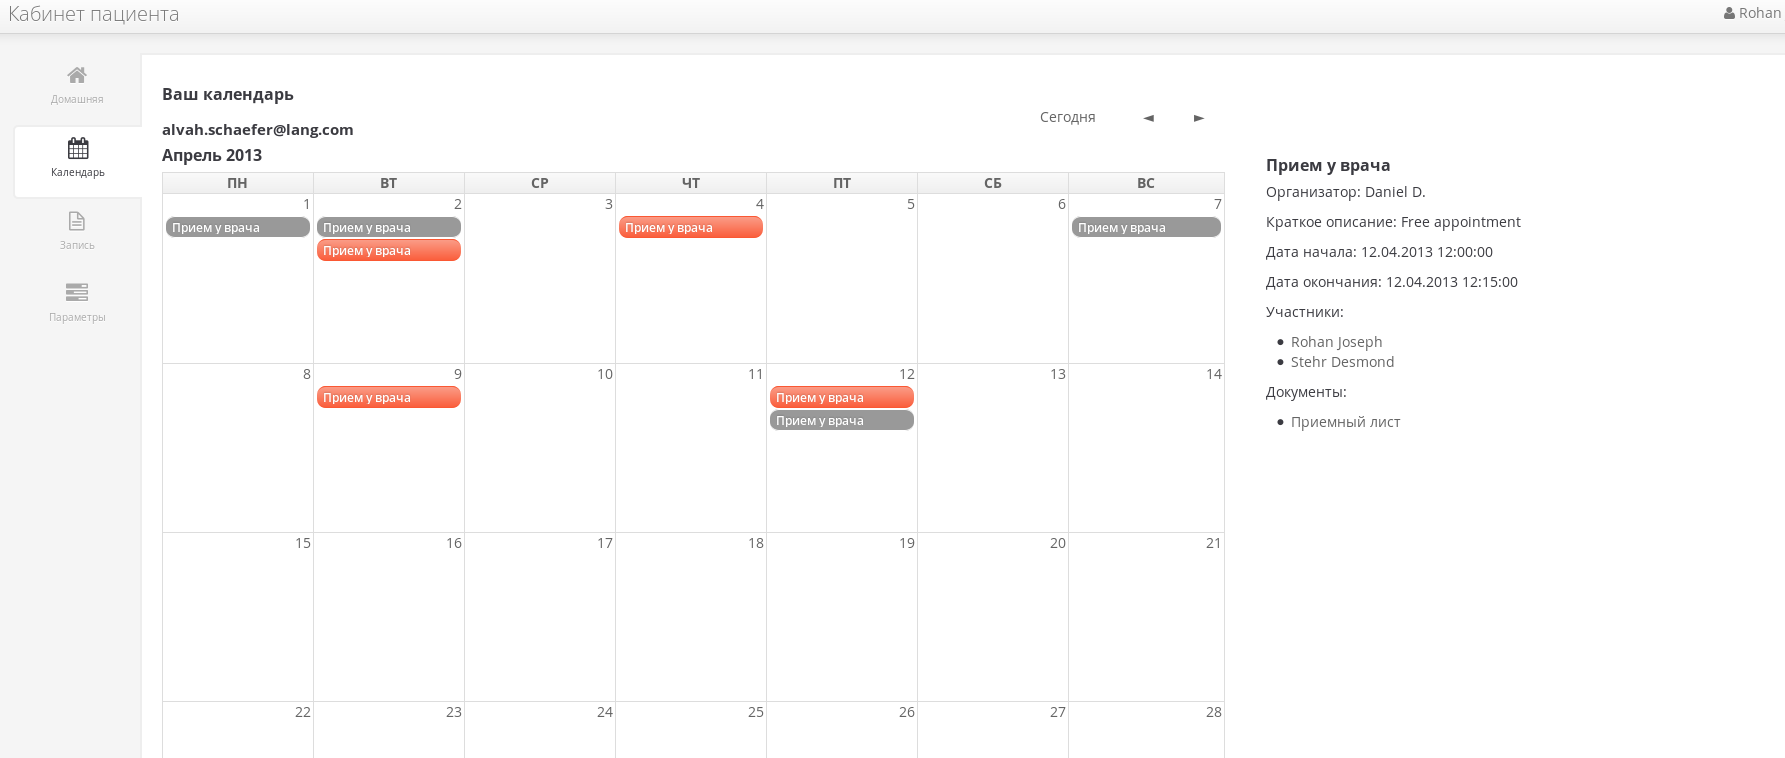
\includegraphics[width=1\linewidth,angle=90]{patient_cabinet_events.eps}}
\caption{Кабинет пациента: список событий}
\label{app:patient_cabinet_events}
\end{figure}

\newpage \begin{figure}[h]
\center{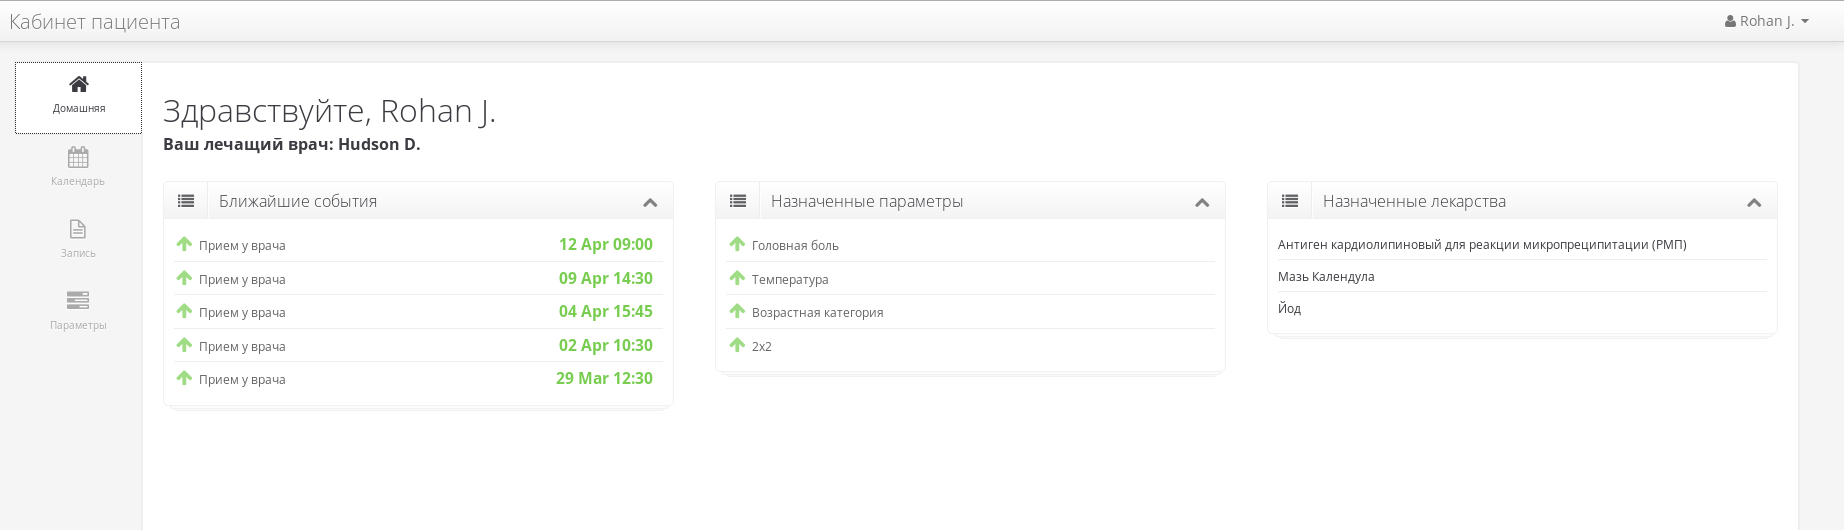
\includegraphics[width=1\linewidth,angle=90]{patient_cabinet_main.eps}}
\caption{Кабинет пациента: главная страница}
\label{app:patient_cabinet_main}
\end{figure}

\newpage \begin{figure}[h]
\center{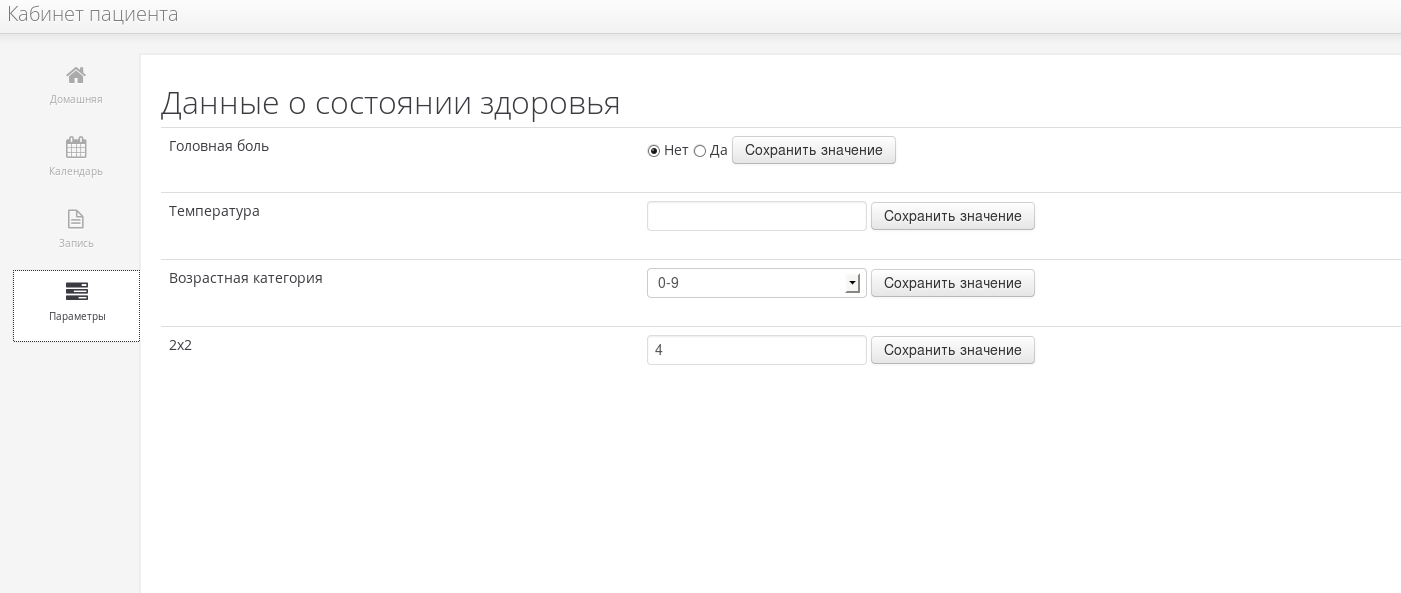
\includegraphics[width=1\linewidth,angle=90]{cabinet_patient_parameters.eps}}
\caption{Кабинет пациента: ввод параметров}
\label{app:patient_cabinet_parameters}
\end{figure}

\newpage \begin{figure}[h]
\center{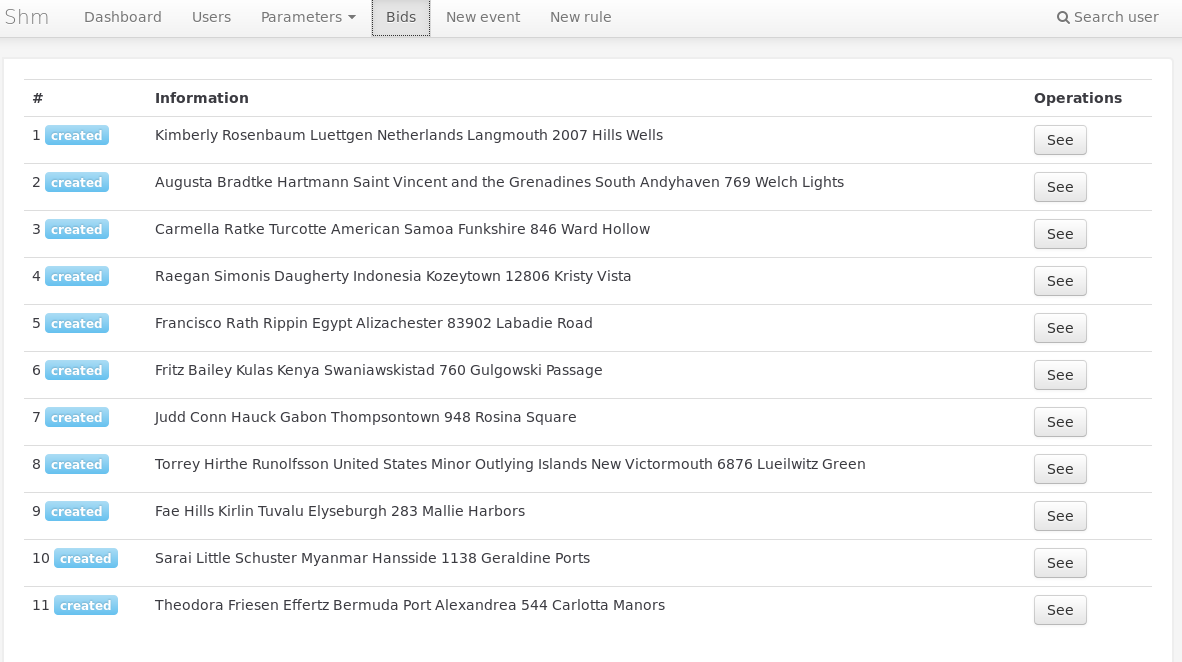
\includegraphics[width=1\linewidth,angle=90]{manager_cabinet_bids.eps}}
\caption{Кабинет менеджера: список заявок}
\label{app:manager_cabinet_bid}
\end{figure}

\newpage \begin{figure}[h]
\center{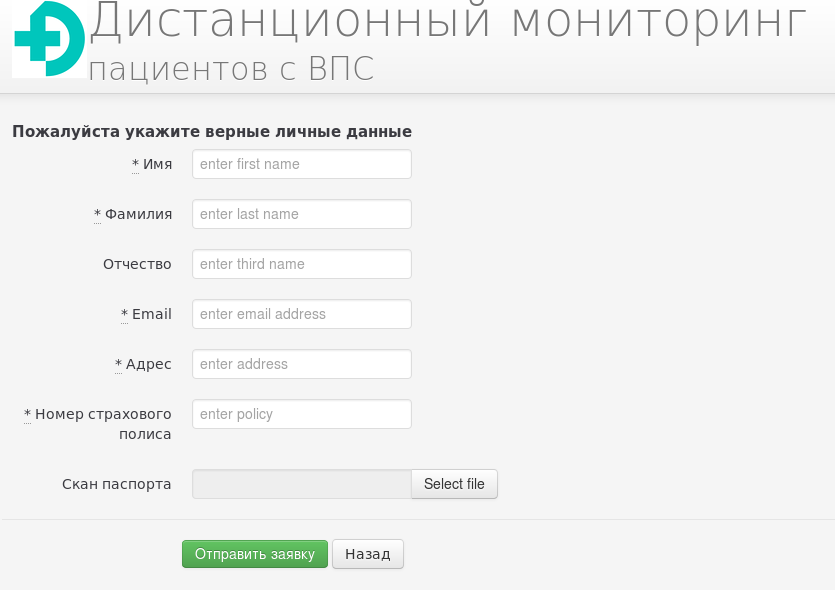
\includegraphics[width=1\linewidth,angle=90]{bid_form.eps}}
\caption{Подача заявки}
\label{app:bid_form}
\end{figure}


\end{document}